\newpage
\vskip 6mm
\pagestyle{myheadings}
\markboth{{\underline{\centerline{东南大学博士学位论文} }}}
{{\underline{\centerline{第二章 \ \ \  两种基于r\'{e}nyi熵的分数阶累计剩余时间序列度量 } }}}

\chapter{两种基于r\'{e}nyi熵的分数阶累计剩余时间序列度量}\label{ch2}
\setcounter{equation}{0}
 
\section{引言}
在信息论中,香农熵(或称信息熵)被提出来衡量随机变量的信息量(cite{1})。给定一个随机变量 $X$,其概率密度函数为 $F(x)$,则 $X$ 的香农熵 (SE) 定义为:
\begin{align}\label{SE}
SE(X)=-\int_{0}^{\infty}F(x)\log F(x)dx,
\end{align}
其中,$\log$ 是以 2 为底的对数。香农熵的离散形式是基于离散概率分布 $P(X)$,给定一个随机变量 $X_{t}=\{x_{1},x_{2},\ldots,x_{t}\}$,相应的概率为 $P(X)=P(x=x_{i}),i=1,2,\ldots,t$,离散香农熵(DSE)可定义为:
\begin{align}\label{DSE}
DSE(X)=-\sum\limits_{i=1}^{t} P(X=x_{i})\log (P(X=x_{i}))dx.
\end{align}
SE的计算公式表明,概率越高,信息的不确定性就越小,而所需信息的预期数量则以比特为单位,用对数来表示。由于其稳健的数学基础和固有的灵活性,SE 在信息检索\cite{2}、数据处理\cite{3}和机器学习\cite{4}等不同领域得到了广泛应用。然而,一些特性限制了 SE 在时间序列分析中的应用。例如,单独计算每个数据点的概率会导致对异常值的敏感性。此外,香农熵只关注每个事件的概率,而忽略了每个事件的值,这使得信息不确定性的计算不可靠。为了解决上述问题,Rao 等人提出了基于生存函数和累积分布函数的累积残差熵\cite{2_5},其定义为:
\begin{align}\label{CRE}
CRE(X_{t})=-\int_{0}^{\infty}\hat F(x)\log \hat F(x)dx,
\end{align}
其中 $\hat F(x)=1-F(x)=P(X\geq x_{i})$ 是生存函数。$\rm{CRE}$ 是 $\rm{SE}$ 的扩展,考虑了概率分布的累积残差。$\rm{CRE}$包含了之前观测的残差信息,而$\rm{SE}$只考虑了当前观测的熵。换句话说,$\rm{CRE}$ 考虑了过去观测值的累积信息,使其成为时间序列中整体不确定性或无序性的度量,同时考虑了历史残差 \cite{6}。
与此类似,CRE 也可以离散形式存在,给定一个非负离散随机过程 $X$,离散累积残差熵($\rm{DCRE}$)可以定义为:
\begin{align}\label{DCRE}
DCRE(X_{t})=-\sum\limits_{i=1}^{t}P(X\geq x_{i})\log P(X\geq x_{i})(x_{i}-x_{i-1}),
\end{align}
其中,$P(X\geq x_{i})$是$X$的累积分布函数($\rm{CDF}$),也可用于计算$P(a < X \leq b)$形式的事件概率,方法是求出在$a$和$b$处评估的CDF之差:$P(X\geq x_{i})$。

在 $\rm{SE}$ 和 $\rm{CRE}$ 的基础上,人们提出了一些度量方法来量化时间序列的各种特征或属性。其中,Kullback-Leibler(KL)散度又称相对熵,是对两个随机变量概率分布之间相似度的一种度量。给定两个随机变量 $X$ 和 $Y$ 的概率分布分别为 $F(x)$ 和 $G(x)$,则 $X$ 和 $Y$ 之间的KL散度 $KL(X,Y)$ 定义为:
\begin{align}\label{KL}
KL(X,Y)=-\int_{0}^{\infty} F(x)\log \frac{F(x)}{G(x)}dx,
\end{align}

KL 散度量化了使用为 $G(x)$ 设计的最佳编码来表示从 $F(x)$ 采样的数据所需的平均额外比特数。它衡量了用一种分布逼近另一种分布时损失或获得的信息。KL 散度总是非负的,而且只有当 $F(X)=G(Y)$ 时,$KL(X,Y) = 0$。基于 $\rm{CRE}$ 的概念,KL 散度可以扩展到累积残差 KL 散度($\rm{CEKL}$)\cite{8}:
\begin{align}\label{KL}
CRKL(X,Y)=-\int_{0}^{\infty} \hat F(x)\log \frac{\hat F(x)}{\hat G(x)}dx,
\end{align}
另一种时间序列度量是传递熵($\rm{TE}$)。传递熵的形式与 KL 散度相似,也可以写成概率分布乘以对数项的形式。与 KL 散度相比,$\rm{TE}$ 是两个随机过程之间信息定向流动的度量,因此,$\rm{TE}$ 通常用于识别因果关系中因果之间的时间阶梯。从数学表达式上来看$\rm{TE}$本质上是与变量历史数据影响的条件互信息(CMI)。给定两个连续的随机过程$X$和$Y$,从$X$到$Y$的$rm{TE}$可以表示为\cite{9}:

\begin{align}\label{TE}
TE_{Y\rightarrow X}=\int_{-\infty}^{\infty} \int_{-\infty}^{\infty} p(x_{t+1}, x_t^{(k)}, y_{t}^{(l)}) \log_{2} \frac{p(x_{t+1}|x_t^{(k)}, y_{t}^{(l)})}{p(x_{t+1}|x_t^{(k)})} dx dy
\end{align}

其中$k$和$l$是马尔可夫阶数,它控制变量$X$和$Y$历史信息的滞后时间。一些研究者在 $rm{TE}$ 中用 $\rm{CDF}$ 代替了 $\rm{PDF}$,以使用 $\rm{CRE}$ 的特性 (cite{10,11,12})。然而,这些工作没有给出累积残余传递熵($\rm{CRTE}$)的正式定义,这促使我们进一步将 $\rm{TE}$ 扩展到具有累计剩余度量性质的 $\rm{CRTE}$。

总之,KL 散度和 $\rm{TE}$ 都是信息传递或流动的度量,但它们在度量这种流动的方法上有所不同。KL 散度测量的是各系统概率分布之间的差异,因此,KL 常被用作距离度量\cite{13,14,15,16}。$\rm{TE}$ 衡量的是系统中变量间信息的定向流动,更适合研究具有时间依赖性的复杂系统,可用于识别系统中因果互动的方向和强度 \cite{17,18,19,20}。

此外,作为SE的分数阶形式扩展,R{\'e}nyi引入了R{\'e}nyi熵(RE)来度量时间序列的复杂性\cite{21}。令 $\alpha \geq 0$,随机变量 $X$的$\alpha$阶RE定义为:
\begin{align}\label{RE}
H_{\alpha}(X) = \dfrac{1}{1 - \alpha} \log_2 \left(\sum_{x \in \mathcal{X}} p(x)^{\alpha} \right)
\end{align}
其中,$X$ 是分布为 $p(x)$ 的离散型随机变量,$\mathcal{X}$ 是$X$ 可能结果的集合。RE 是一个关于 $\alpha$ 的非负的、单调递减的函数\cite{22}。根据 L'Hospital 规则,当 $\alpha=1$ 时,RE 收敛到 SE。当 $alpha \geq 1$ 时,RE 更偏向于代表变量 $X$ 分布中的高频事件。当 $\alpha=2$ 时,RE转换为 $\rm{collision\ entropy}$;当 $\alpha=+\infty$ 时,RE转换为 $\rm{minimum\ entropy}$。此外,当 $\alpha \leq 1$时,RE 中强调的是 $X$ 的低频事件,而当 $\alpha > 1$ 时,强调的是 $X$ 中的高频事件\cite{23}。与传统的 $\rm{SE}$ 相比,$\rm{RE}$ 能够根据需要自适应地测量复杂分布。由于R\'{e}nyi熵在复杂分布上的有效性,一些研究者将KL散度和$\rm{TE}$扩展到了分数阶\cite{24,25},即所谓的R\'{e}nyi散度($\rm{RKL}$)和R\'{e}nyi传递熵($\rm{RTE}$)。这些工作也启发我们在 RE 的基础上将 $\rm{CRKL}$ 和 $\rm{CRTE}$ 扩展到分数阶,从而更全面地衡量时间序列之间的关系。

综上,本章引入了两种分数阶累积剩余时间序列度量,分别称为r\'{e}nyi cumulative residual kullback-leibluer ($\rm{RCRKL}$)和r\'{e}nyi cumulative residual transfer entropy ($\rm{RCRTE}$)。这两种度量方法都基于累积残差熵和r/'{e}nyi熵,其中$\rm{RCRKL}$主要用于比较时间序列之间的相似性,而$\rm{RCRTE}$则用于分析时间序列数据中的信息流和变量之间的因果关系。同时,我们证明了 $\rm{RCRKL}$ 作为距离度量的一些性质,并研究了 $\rm{RCRTE}$ 的零点和边界。为了验证本章所提出度量的有效性,我们分别在仿真数据和真实数据上进行了数值验证。在仿真数据的验证部分,我们研究了参数变换对两种度量的影响。在真实数据验证部分,我们采用了来自RIOHTrack的路面车辙数据,基于RCRKL作为距离度量,设计了一种新型的聚类算法,对不同路面的车辙进行聚类,并基于RCRTE对每个簇里的车辙进行因果关系检测。结果显示,基于RCRKL的聚类算法具有良好的聚类性能,而RCRTE也能有效检测出显著的因果关系。

\section{R\'{e}nyi 累积剩余KL散度及其性质}

\textbf{定义 1.} 给定两个随机变量 $X$ 和 $Y$。R\'{e}nyi cumulative residual kullback-leibluer divergence($\rm{RCRKL}$)的定义是:
\begin{align}
RCRKL(X,Y)=\frac{1}{\alpha-1} \log \left( \int_{-\infty}^{\infty} \hat F(x)^{\alpha} \hat G(y)^{1-\alpha} dx \right),
\end{align}

在这个公式中,$\hat F(x)$ 表示随机变量 $X$ 的生存函数,$\hat G(y)$ 表示随机变量 $Y$ 的生存函数。

在本节接下来的内容中,将提供 CRKL 的一些一般性质和相应的证明。

\textbf{命题 1.} 令 $X$ 和 $Y$ 是两个随机变量,并且 $\alpha\ge 1$,那么
\begin{align*}
RCRKL(X,Y)\geq 0,
\end{align*}

\textbf{证明}\\
首先,回顾$\rm{RCRKL}$公式为:
\begin{align*}
RCRKL(X,Y)=\frac{1}{\alpha-1} \log \left( \int_{-\infty}^{\infty} \hat F(x)^{\alpha} \hat G(y)^{1-\alpha} dx \right),
\end{align*}
由于 $\alpha \geq 1$,分母 $\alpha - 1$ 是非负数。因此,只证明证明$\rm{RCRKL}$中的对数项大于1 ,即:
\begin{align*}
\int_{-\infty}^{\infty} \hat{F}(x)^{\alpha} \hat{G}(y)^{1-\alpha} dx \geq 1.
\end{align*}

根据定义\cite{111},生存函数 $\hat{F}(x)$ 和 $\hat{G}(y)$ 是非负值,其值介于 0 和 1 之间。 因此,通过应用广义的 H\"{o}lder 不等式,我们可以得到下面的不等式:
\begin{align*}
\int_{-\infty}^{\infty} \hat{F}(x)^{\alpha} \hat{G}(y)^{1-\alpha} dx &\geq \left(\int_{-\infty}^{\infty} \hat{F}(x) dx \right)^{\alpha} \left(\int_{-\infty}^{\infty} \hat{G}(y) dy \right)^{1-\alpha}.
\end{align*}
同时,生存函数 $\hat{F}(x)$ 和 $\hat{G}(y)$ 的此积分为 1,即:
\begin{align*}
\int_{-\infty}^{\infty} \hat{F}(x) dx = \int_{-\infty}^{\infty} \hat{G}(y) dy= 1,
\end{align*}
将这些值代入上一不等式,我们得出:
\begin{align*}
\int_{-\infty}^{\infty} \hat{F}(x)^{\alpha} \hat{G}(y)^{1-\alpha} dx &\geq 1^{\alpha} \cdot 1^{1-\alpha} \\
&= 1.
\end{align*}

因此,我们得出结论:$RCRKL(X, Y) \geq 0$ for $\alpha \geq 1$。

证明完毕。\\

\textbf{命题 2.} 令 $X$ 和 $Y$为两个随机变量,$a,b,$ 和 $c$为常数,那么
\begin{align*}
RCRKL(aX+b,cY+b)=a\cdot RCRKL(X,\frac{c}{a}Y),
\end{align*}
其中 $\hat F(x)$ 表示随机变量 X 的生存函数,$\hat G(x)$ 表示随机变量 Y 的生存函数。

\textbf{证明}\\
首先,考虑待证等式:
\begin{align*}
RCRKL(aX+b,cY+b)=a\cdot RCRKL(X,\frac{c}{a}Y),
\end{align*}
将 $\rm{RCRKL}$公式代入 LHS,可得:
\begin{align*}
RCRKL(aX+b,cY+b) &=\frac{1}{\alpha-1} \log \left(\int_{-\infty}^{\infty}\hat F^{\alpha}(aX+b)\hat G^{1-\alpha}(cY+b)dx \right),\\
&= \frac{1}{\alpha-1} \log \left(\int_{-\infty}^{\infty}\hat F_{aX+b}(x)^{\alpha} \hat G_{cY+b}(x )^{1-\alpha}dx \right),\\
\end{align*}

令 $u=aX+b$ and $v=cY+b$,则上式可写为:
\begin{align*}
RCRKL(aX+b,cY+b) &=\frac{1}{\alpha-1} \log \left(\int_{-\infty}^{\infty}\hat F_{\frac{1}{a}(u-b)}(x)^{\alpha}\hat G_{\frac{1}{a}(v-b)}(y)^{1-\alpha}dx \right)\\
\end{align*}

再将带证等式RHS中变量$X$和$Y$替换为$u$和$v$,可得:
\begin{align*}
a\cdot RCRKL(X,\frac{c}{a}Y) &=a\cdot \frac{1}{\alpha-1} \log \left(\int_{-\infty}^{\infty}\hat F_{X}(x)^{\alpha}\hat G_{\frac{c}{a}Y}(x)^{1-\alpha}dx \right)\\
&=\frac{1}{\alpha-1} \log \left(\int_{-\infty}^{\infty}\hat F_{\frac{1}{a}(u-b)}(x)^{\alpha}\hat G_{\frac{1}{a}(v-b)}(y^{1-\alpha})dx \right)\\
\end{align*}
显然,$\rm{LHS}=\rm{RHS}$。因此,我们有:
$$RCRKL(aX+b,cY+b)=a\cdot RCRKL(X,\frac{c}{a}Y), $$

证明完毕。\\

\textbf{命题3.} 令 $X$ 和 $Y$为两个随机变量,$0\leq \lambda \leq 1$ 且 $\alpha \geq 0$,则:$$RCRKL(\lambda X_{1}+(1-\lambda) X_{2}, \lambda Y_{1}+(1-\lambda)Y_{2}) \leq \lambda RCRKL(X_{1},Y_{1})+(1-\lambda) RCRKL(X_{2},Y_{2}).\\$$

\textbf{证明}\\
令 $Z_{1}=\lambda X_{1}+(1-\lambda) X_{2}$ 及 $W_{1}=\lambda Y_{1}+(1-\lambda)Y_{2},$ 其中 $0\leq \lambda \leq 1.\\$

那么,$Z_{1}$ 和 $W_{1}$ 之间的 $\rm{RCRKL}$ 可以表示为:

$$RCRKL(Z,W) = \frac{1}{\alpha-1}\log_{2}\int_{-\infty}^{\infty} \hat F_{Z_{1}}(x)^{\alpha} \hat G_{W_{1}}(x)^{1-\alpha} \lambda dx),\\$$
利用生成函数的性质,我们可以得到:
\begin{align*}
\hat F_{Z_{1}}(x) &= P(Z_{1} \geq x)\\
&= P(\lambda X_{1}+(1-\lambda) X_{2}\geq x)\\
&\leq \lambda P(X_{1}\geq x)+ (1-\lambda) P(X_{2}\geq x)\\
&= \lambda \hat F_{X_{1}}(x)+ (1-\lambda) \hat F_{X_{2}}(x)
\end{align*}

类似的,我们有:
\begin{align*}
\hat G_{W_{1}}(x) \leq \lambda \hat F_{Y_{1}}(x)+ (1-\lambda) \hat F_{Y_{2}}(x),
\end{align*}

将这些不等式代入 $\rm{RCRKL}$ 公式,即可得出:
\begin{align*}
RCRKL(Z_{1},W_{1})\leq \frac{1}{\alpha -1}\log_{2}(\int_{-\infty}^{\infty}(\lambda \hat F_{X_{1}}(x)+(1-\alpha)\hat F_{X_{2}}(x))^{\alpha})(\lambda \hat G_{Y_{1}}(x)+(1-\alpha)\hat G_{Y_{2}}(x))^{1-\alpha}dx),
\end{align*}

利用对数性质,我们可以简化上式:
\begin{align*}
RCRKL(Z_{1},W_{1})\leq \lambda \cdot RCRKL(X_{1},Y_{1}) +(1-\lambda) \cdot RCRKL(X_{2},Y_{2}).
\end{align*}

因此,可以证明到:
\begin{align*}
RCRKL(\lambda X_{1}+(1-\lambda)X_{2}, \lambda Y_{1}+(1-\lambda)Y_{2})\leq \lambda \cdot RCRKL(X_{1},Y_{1}) +(1-\lambda) \cdot RCRKL(X_{2},Y_{2}),
\end{align*}
对于$0\leq \lambda \leq 1$范围内的任何$\lambda$值和任何$\alpha \geq 0$来说都成立。

证明完毕。\\

\textbf{命题 4.} 当$\alpha \ge 1$时,$\rm{RCRKL}$满足三角不等式,即:
$$RCRKL(X,Y) + RCRKL(Y,Z) \ge RCRKL(X,Z)$$

\textbf{证明}\\
利用 $\rm{RCRKL}$ 散度的定义,我们可以把 LHS 写成:
\begin{align*}\
RCRKL(X,Y) + RCRKL(Y,Z) &= \frac{1}{\alpha - 1}\log (\int_{-\infty}^{\infty} \hat F_{X}^{\alpha}(x) \int_{-\infty}^{\infty} \hat G_{Y}^{1-\alpha}(x)dx)\\
 &+ \frac{1}{\alpha - 1}\log (\int_{-\infty}^{\infty} \hat F_{Y}^{\alpha}(y) \int_{-\infty}^{\infty} \hat G_{Z}^{1-\alpha}(y)dy),
\end{align*}

而 RHS 可以写成:
\begin{align*}\
RCRKL(X,Z) = \frac{1}{\alpha - 1}\log (\int_{-\infty}^{\infty} \hat F_{X}^{\alpha}(x) \int_{-\infty}^{\infty} \hat G_{Z}^{1-\alpha}(x)dx).
\end{align*}

我们首先考虑$\rm{RCRKL}$散度内部的对数项,根据 Cauchy-Schwarz不等式,我们可以得到:
\begin{align*}\
\sqrt{\int_{-\infty}^{\infty} \hat F_{X}^{\alpha}(x) \int_{-\infty}^{\infty} \hat G_{Y}^{1-\alpha}(x)dx}\cdot \sqrt{\int_{-\infty}^{\infty} \hat F_{Y}^{\alpha}(y) \int_{-\infty}^{\infty} \hat G_{Z}^{1-\alpha}(y)dy} \ge  \int_{-\infty}^{\infty} \hat F_{X}^{\alpha}(x) \int_{-\infty}^{\infty} \hat G_{Z}^{1-\alpha}(x)dx.
\end{align*}

将不等式两边平方,就得到:
\begin{align*}\
\int_{-\infty}^{\infty} \hat F_{X}^{\alpha}(x) \int_{-\infty}^{\infty} \hat G_{Y}^{1-\alpha}(x)dx \cdot \int_{-\infty}^{\infty} \hat F_{Y}^{\alpha}(y) \int_{-\infty}^{\infty} \hat G_{Z}^{1-\alpha}(y)dy \ge  (\int_{-\infty}^{\infty} \hat F_{X}^{\alpha}(x) \int_{-\infty}^{\infty} \hat G_{Z}^{1-\alpha}(x)dx)^{2}.
\end{align*}

对两边取对数,我们有:
\begin{align*}\
\log(\int_{-\infty}^{\infty} \hat F_{X}^{\alpha}(x) \int_{-\infty}^{\infty} \hat G_{Y}^{1-\alpha}(x)dx)+ \log(\int_{-\infty}^{\infty} \hat F_{Y}^{\alpha}(y) \int_{-\infty}^{\infty} \hat G_{Z}^{1-\alpha}(y)dy) \ge 2\log (\int_{-\infty}^{\infty} \hat F_{X}^{\alpha}(x) \int_{-\infty}^{\infty} \hat G_{Z}^{1-\alpha}(x)dx).
\end{align*}

当 $alpha \ge 1$ 时,我们可以得到:
\begin{align*}\
&\frac{1}{\alpha-1}\log(\int_{-\infty}^{\infty} \hat F_{X}^{\alpha}(x) \int_{-\infty}^{\infty} \hat G_{Y}^{1-\alpha}(x)dx)+ \frac{1}{\alpha-1}\log(\int_{-\infty}^{\infty} \hat F_{Y}^{\alpha}(y) \int_{-\infty}^{\infty} \hat G_{Z}^{1-\alpha}(y)dy) \ge\\
& \frac{2}{\alpha-1}\log (\int_{-\infty}^{\infty} \hat F_{X}^{\alpha}(x) \int_{-\infty}^{\infty} \hat G_{Z}^{1-\alpha}(x)dx).
\end{align*}

因此,我们证明了
\begin{align*}\
RCRKL(X,Y) +RCRKL(Y,Z) \ge 2 RCRKL(X, Z)).
\end{align*}

又因为当$\alpha \ge 1$时, $RCRKL(X,Y) \ge 0$, 因此我们有:
\begin{align*}\
RCRKL(X,Y) +RCRKL(Y,Z) \ge  RCRKL(X, Z).
\end{align*}
证明完毕。\\

\section{R\'{e}nyi累积剩余传递熵及其性质}
首先,我们先介绍累积残余传递熵(Cumulative Residual Transfer Entropy,$\rm{CRTE}$)的定义,$\rm{CRTE}$ 是传递熵(Transfer Entropy,$\rm{TE}$)的扩展,它将累积剩余熵(cumulative residual entropy,$\rm{CRE}$)的概念纳入到两个离散马尔可夫过程之间的信息传递或因果关系的计算中。$\rm{CRTE}$量化了在考虑了两个过程的历史依赖性的影响之后,根据另一个过程的过去历史预测一个过程的未来状态的累积剩余熵。
\textbf{定义 2.} 给定两个随机变量$X$和$Y$,从$Y$到$X$的$\rm{CRTE}$被表示为:
\begin{align}\label{CRTE}
CRTE(Y \rightarrow X) = -\int_{0}^{\infty} \int_{0}^{\infty} \hat{F}(x_{t+1}|x_t^{(k)}, y_{t}^{(l)}) \log_{2} \frac{\hat{F}(x_{t+1}|x_t^{(k)}, y_{t}^{(l)})}{\hat{F}(x_{t+1}|x_{t}^{(k)})}  dx dy,
\end{align}

基于$\rm{CRTE}$的形式,我们再给出R\'{e}nyi 累积残余传递熵(R\'{e}nyi cumulative residual transfer entropy,$\rm{RCRTE}$)的定义:

\textbf{定义 3.}将\ref{RE}中的 $H_{alpha}$ 代入 \ref{CCRTE},$\rm{CRTE}$可以扩展到分数阶,其定义为 R\'{e}nyi 累积残差传递熵,$\rm{RCRTE}$:
\begin{align}\label{CRTEc}
RCRETE(Y \rightarrow X) = \frac{1}{{1 - \alpha}} \log_{2} \left[ \frac{\int  \rho_{\alpha}(x_t^l)  \hat F^{\alpha}(x_{t+1} | x_t^l)  dx }{\int \int \rho_{\alpha}(x_t^l, y_t^k)  \hat F^{\alpha}(x_{t+1} | x_t^l, y_t^k)  dx  dy} \right]
\end{align}
其中,$\rho_{\alpha}(x)=\frac{\hat F^{\alpha}(x)}{\int\hat F^{\alpha}(x)dx}$为分配分布。

同时,与传统的传递熵类似,$rm{CRTE}$ 也是一个非对称度量。因此,为了表示 $\rm{CRTE}$ 的方向性,方程\ref{CRTEc}也可以改写成条件熵差的形式:
\begin{align}\label{CCRTE}
RCRTE(Y \rightarrow X) &= RCRE(x_{t+1}|x_{t}^{(l)})-RCRE(x_{t+1}|x_{t}^{(l)},y_{t}^{k})\\
&=RCRE(x_{t+1},x_{t}^{(l)})-RCRE(x_{t}^{(l)})+RCRE(x_{t+1},x_{t}^{(l)},y_{t}^{(k)})-RCRE(x_{t}^{(l)},y_{t}^{(k)})
\end{align}
其中,$CRE(X|Y)$ 是条件累积残差熵,它表示了与$Y$ 相同的概率质量函数;$RCRE(X,Y)$ 是联合累积残差熵,与$p(y_{t})$ 相关联的结果对应于以$Y=y_{i}$ 为条件的概率累积残差熵,即$CRE(X|Y=y_{i})$。

此外,离散的R\'{e}nyi 累积残差传递熵(discrete r\'{e}nyi cumulative residual transfer entropy,$\rm{DRCRTE}$)可以定义为:
\begin{align}
DRCRTE_{Y \rightarrow X}^\alpha = \frac{1}{{1 - \alpha}} \log_{2} \left[ \frac{\sum\limits_{x\in X} \rho_{\alpha}(x_{t}^{(l)}) \cdot F^{\alpha}(x_{t+1}|x_t^{(l)}) }{\sum\limits_{y\in Y} \sum\limits_{x\in X} \rho_{\alpha}(x_{t}^{(l)}, y_{t}^{(k)}) \cdot \hat F^{\alpha}(x_{t+1}|x_t^{(k)}, y_{t}^{(l)})} \right].
\end{align}

在本节的其余部分,我们将给出$\rm{RCRTE}$的一些性质和证明:

\textbf{命题 5.} $\rm{RCRTE}$ 随着 $\alpha$ 的增加而单调递减。

首先,观察$\rm{RCRTE}$的定义可知,为了证明 $\rm{RCRTE}$ 随 $\alpha$ 的增加而单调递减,我们需要证明 $\rm{RCRTE}$ 中对数项的随 $\alpha$ 的增加而递减。

$\rm{RCRTE}$ 的定义公式为:
\begin{align*}
RCRTE(Y \rightarrow X) = \frac{1}{1-\alpha} \log \left( \frac{\int_{0}^{\infty}\hat F^{\alpha}(x_{t+1},x_{t}^{(l)})dx \int_{0}^{\infty}\int_{0}^{\infty}\hat F^{\alpha}(x_{t+1},x_{t}^{(l)},y_{t}^{(k)})dxdy}{\int_{0}^{\infty}\hat F^{\alpha}(x_{t}^{l})dx \int_{0}^{\infty}\int_{0}^{\infty}\hat F^{\alpha}(x_{t}^{(l)},y_{t}^{(k)})dxdy} \right)
\end{align*}

我们将把对数中的分子和分母分别记为 $N(\alpha)$ 和 $D(\alpha)$,则有:

\begin{align*}
N(\alpha) &= \int_{0}^{\infty}\hat F^{\alpha}(x_{t+1},x_{t}^{(l)})dx \int_{0}^{\infty}\int_{0}^{\infty}\hat F^{\alpha}(x_{t+1},x_{t}^{(l)},y_{t}^{(k)})dxdy\\
D(\alpha) &= \int_{0}^{\infty}\hat F^{\alpha}(x_{t}^{(l)})dx \int_{0}^{\infty}\int_{0}^{\infty}\hat F^{\alpha}(x_{t}^{(l)},y_{t}^{(k)})dxdy
\end{align*}

利用对数求和不等式,我们可以得出:对于任何正数 a 和 b:
\begin{align*}
\log(a) - \log(b) \leq \frac{a-b}{b}
\end{align*}

将这一不等式应用于 $N(\alpha)$ 和 $D(\alpha)$,我们得到:
\begin{align*}
\log\left(\frac{N(\alpha_2)}{D(\alpha_2)}\right) - \log\left(\frac{N(\alpha_1)}{D(\alpha_1)}\right) \leq \frac{\frac{N(\alpha_2)}{D(\alpha_2)} - \frac{N(\alpha_1)}{D(\alpha_1)}}{\frac{N(\alpha_1)}{D(\alpha_1)}}
\end{align*}

将不等式右侧简化,我们有:
\begin{align*}
\log\left(\frac{N(\alpha_2)}{D(\alpha_2)}\right) - \log\left(\frac{N(\alpha_1)}{D(\alpha_1)}\right) &\leq \frac{\frac{N(\alpha_2)}{D(\alpha_2)} - \frac{N(\alpha_1)}{D(\alpha_1)}}{\frac{N(\alpha_1)}{D(\alpha_1)}}\\
& \leq \frac{N(\alpha_2)D(\alpha_1) - N(\alpha_1)D(\alpha_2)}{D(\alpha_1)N(\alpha_1)}\\
&= \frac{N(\alpha_2)}{N(\alpha_1)} - \frac{D(\alpha_2)}{D(\alpha_1)}
\end{align*}

由于 $\alpha_1 < \alpha_2$, 则 $\frac{N(\alpha_2)}{N(\alpha_1)} \leq 1$ and $\frac{D(\alpha_2)}{D(\alpha_1)} \geq 1$.

因此,我们可以得出:
\begin{align*}
\log\left(\frac{N(\alpha_2)}{D(\alpha_2)}\right) - \log\left(\frac{N(\alpha_1)}{D(\alpha_1)}\right) \leq \frac{N(\alpha_2)}{N(\alpha_1)} - \frac{D(\alpha_2)}{D(\alpha_1)} \leq 0
\end{align*}
由于对数是单调递增函数,上述不等式意味着 $\frac{N(\alpha_2)}{D(\alpha_2)} \leq \frac{N(\alpha_1)}{D(\alpha_1)}$。
因此,我们可以得出结论,$\rm{RCRTE}$随着 $\alpha$ 的增加而单调递减。

证明完毕。\\

\textbf{命题 6.} 令 $X$ 和 $Y$为两个随机变量,那么当且仅当随机变量 X 和 Y 的分布处处相同时,$\rm{RCRTE}(Y \rightarrow X) = 0$。

要证明 $\rm{RCRTE}(Y \rightarrow X) = 0$ 当且仅当 X 和 Y 的分布处处相同时,我们需要证明该命题的充要性。

充分性:$\rm{RCRTE}(Y \rightarrow X) = 0$ 意味着 X 和 Y 的分布处处相同。
	
\textbf{证明}\\

如果 $\rm{RCRTE}(Y\rightarrow X) = 0$,那么根据 $\rm{RCRTE}$ 的定义,我们有:
\begin{align*}
\frac{1}{1-\alpha} \log \left( \frac{\int_{0}^{\infty}\hat F^{\alpha}(x_{t+1},x_{t}^{(l)})dx \int_{0}^{\infty}\int_{0}^{\infty}\hat F^{\alpha}(x_{t+1},x_{t}^{(l)},y_{t}^{(k)})dxdy}{\int_{0}^{\infty}\hat F^{\alpha}(x_{t}^{l})dx \int_{0}^{\infty}\int_{0}^{\infty}\hat F^{\alpha}(x_{t}^{(l)},y_{t}^{(k)})dxdy} \right) = 0
\end{align*}

这意味着该分数项的分子等于分母,即:
\begin{align*}
\int_{0}^{\infty}\hat F^{\alpha}(x_{t+1},x_{t}^{(l)})dx \int_{0}^{\infty}\int_{0}^{\infty}\hat F^{\alpha}(x_{t+1},x_{t}^{(l)},y_{t}^{(k)})dxdy = \int_{0}^{\infty}\hat F^{\alpha}(x_{t}^{l})dx \int_{0}^{\infty}\int_{0}^{\infty}\hat F^{\alpha}(x_{t}^{(l)},y_{t}^{(k)})dxdy
\end{align*}
由于累积分布函数(CDF)$\hat F$ 表示随机变量大于或等于某个值的概率,因此积分相等意味着联合 CDF $\hat F(x_{t}^{(l)},y_{t}^{(k)})$ 等于边际 CDF $\hat F(x_{t}^{l})$ 和 $\hat F(x_{t}^{(l)})$ 的乘积。\\
因此,我们可以得出结论:如果 $\rm{RCRTE}(Y \rightarrow X) = 0$,那么 X 和 Y 的分布处处相同。


必要性: X 和 Y 的分布处处相同意味着 $\rm{RCRTE}(Y\rightarrow X) = 0$。

\textbf{证明}\\

如果 X 和 Y 在所有地方都有相同的分布,这意味着它们的联合 CDF $\hat F(x_{t}^{(l)},y_{t}^{(k)})$ 等于它们的边际 CDF $\hat F(x_{t}^{(l)})$ 和 $\hat F(y_{t}^{(k)})$ 的乘积。

因此,我们有:
\begin{align*}
\hat F(x_{t}^{(l)},y_{t}^{(k)}) = \hat F(x_{t}^{(l)}) \cdot \hat F(y_{t}^{(k)})
\end{align*}
考虑到$\rm{RCRTE}$中的每一项,我们有:
\begin{align*}
&\int_{0}^{\infty}\hat F^{\alpha}(x_{t+1},x_{t}^{(l)})dx = \int_{0}^{\infty}(\hat F(x_{t+1},x_{t}^{(l)}))^{\alpha}dx,\\
&\int_{0}^{\infty}\hat F^{\alpha}(x_{t+1},x_{t}^{(l)},y_{t}^{(k)})dxdy = \int_{0}^{\infty}\int_{0}^{\infty}(\hat F(x_{t+1},x_{t}^{(l)},y_{t}^{(k)}))^{\alpha}dxdy,\\
&\int_{0}^{\infty}\hat F^{\alpha}(x_{t}^{(l)})dx = \int_{0}^{\infty}(\hat F(x_{t}^{(l)}))^{\alpha}dx,\\
&\int_{0}^{\infty}\int_{0}^{\infty}\hat F^{\alpha}(x_{t}^{(l)},y_{t}^{(k)})dxdy = \int_{0}^{\infty}\int_{0}^{\infty}(\hat F(x_{t}^{(l)},y_{t}^{(k)}))^{\alpha}dxdy.\\
\end{align*}
现在,把边际 CDF 的表达式代入联合 CDF,我们就得到了:
\begin{align*}
(\hat F(x_{t+1},x_{t}^{(l)}))^{\alpha} = (\hat F(x_{t+1},x_{t}^{(l)}))^{\alpha} \cdot (\hat F(y_{t}^{(k)}))^{\alpha},
\end{align*}
以及
\begin{align*}
(\hat F(x_{t}^{(l)}))^{\alpha} = (\hat F(x_{t}^{(l)}))^{\alpha} \cdot (\hat F(y_{t}^{(k)}))^{\alpha}
\end{align*}
由于指数 $\alpha$ 不为零,我们可以将方程两边分别除以公因子 $(\hat F(x_{t+1},x_{t}^{(l)}))^{\alpha}$ 和 $(\hat F(x_{t}^{(l)}))^{\alpha}$ ,从而得到:
\begin{align*}
(\hat F(y_{t}^{(k)}))^{\alpha} = 1
\end{align*}
由于指数 $\alpha$ 不为零,这些等式成立的唯一条件是 $(\hat F(y_{t}^{(k)}))^{alpha} = 1$,这意味着 $\hat F(y_{t}^{(k)}) = 1$。这意味着随机变量 Y 是一个概率为 1 的常数。
因此,如果 X 和 Y 的分布处处相同,则有 $\rm{RCRTE}(Y \rightarrow X) = 0$。

证明完毕。\\

\textbf{命题 7.} 令$X$ 和 $Y$ 是两个随机变量,且 $l=k=t$,则有:
\begin{align*}1- (\frac{\mathbb{E}(x_{t+1},x_{t}^{(l)})\cdot \mathbb{E}(x_{t+1},x_{t}^{(l)},y_{t}^{(k)})}{\mathbb{E}(x_{t}^{(l)})\mathbb{E}(x_{t}^{(l)},y_{t}^{(k)})})^{\frac{1-\alpha}{\alpha}} &\leq RCRTE(Y \rightarrow X)\\ &\leq (\frac{\mathbb{E}(x_{t+1},x_{t}^{(l)})\cdot \mathbb{E}(x_{t+1},x_{t}^{(l)},y_{t}^{(k)})}{\mathbb{E}(x_{t}^{(l)})\mathbb{E}(x_{t}^{(l)},y_{t}^{(k)})})^{\frac{\alpha}{1-\alpha}}-1
\end{align*}
\textbf{证明.}\\
根据定义,$RCRTE(Y\rightarrow X)$ 的公式可改写为:
\begin{align*}
RCRTE(Y \rightarrow X)&=RCRE(x_{t+1},x_{t}^{(l)})-RCRE(x_{t}^{(l)})+RCRE(x_{t+1},x_{t}^{(l)},y_{t}^{(k)})-RCRE(x_{t}^{(l)},y_{t}^{(k)})\\
&=\frac{1}{1-\alpha}\log \frac{\int_{0}^{\infty}\hat F^{\alpha}(x_{t+1},x_{t}^{l})dx \int_{0}^{\infty}\int_{0}^{\infty}\hat F^{\alpha}(x_{t+1},x_{t}^{(l)},y_{t}^{(k)})dxdy}{\int_{0}^{\infty}\hat F^{\alpha}(x_{t}^{l})dx \int_{0}^{\infty}\int_{0}^{\infty}\hat F^{\alpha}(x_{t}^{(l)},y_{t}^{(k)})dxdy}\\
&= \log \frac{(\mathbb{E}^{\alpha}(x_{t+1},x_{t}^{(l)})\cdot \mathbb{E}^{\alpha}(x_{t+1},x_{t}^{(l)},y_{t}^{(k)}))^{1-\alpha}}{(\mathbb{E}^{\alpha}(x_{t}^{(l)})\mathbb{E}^{\alpha}(x_{t}^{(l)},y_{t}^{(k)}))^{1-\alpha}}\\
&= \log \frac{\mathbb{E}^{\frac{\alpha}{1-\alpha}}(x_{t+1},x_{t}^{(l)})\cdot \mathbb{E}^{\frac{\alpha}{1-\alpha}}(x_{t+1},x_{t}^{(l)},y_{t}^{(k)})}{\mathbb{E}^{\frac{\alpha}{1-\alpha}}(x_{t}^{(l)})\mathbb{E}^{\frac{\alpha}{1-\alpha}}(x_{t}^{(l)},y_{t}^{(k)})}
\end{align*}

由于当 $\alpha \ge 0, \alpha \neq 1$, and $x\ge0$时,有$\log^{\alpha}(x)\leq x-1$,那么我们有:
\begin{align*}
RCRTE(Y \rightarrow X)&= \log \frac{\mathbb{E}^{\frac{\alpha}{1-\alpha}}(x_{t+1},x_{t}^{(l)})\cdot \mathbb{E}^{\frac{\alpha}{1-\alpha}}(x_{t+1},x_{t}^{(l)},y_{t}^{(k)})}{\mathbb{E}^{\frac{\alpha}{1-\alpha}}(x_{t}^{(l)})\mathbb{E}^{\frac{\alpha}{1-\alpha}}(x_{t}^{(l)},y_{t}^{(k)})}\\
& \leq \frac{\mathbb{E}^{\frac{\alpha}{1-\alpha}}(x_{t+1},x_{t})\cdot \mathbb{E}^{\frac{\alpha}{1-\alpha}}(x_{t+1},x_{t},y_{t})-\mathbb{E}^{\frac{\alpha}{1-\alpha}}(x_{t})\cdot \mathbb{E}^{\frac{\alpha}{1-\alpha}}(x_{t},y_{t})}{\mathbb{E}^{\frac{\alpha}{1-\alpha}}(x_{t})\cdot \mathbb{E}^{\frac{\alpha}{1-\alpha}}(x_{t},y_{t})}\\
&=(\frac{\mathbb{E}(x_{t+1},x_{t}^{(l)})\cdot \mathbb{E}(x_{t+1},x_{t}^{(l)},y_{t}^{(k)})}{\mathbb{E}(x_{t}^{(l)})\mathbb{E}(x_{t}^{(l)},y_{t}^{(k)})})^{\frac{\alpha}{1-\alpha}}-1
\end{align*}

不等式右侧得证。

又由于由于当$\alpha \ge 0, \alpha \neq 1$, 且 $x\ge0$ 时, 有$\log_{\alpha}(x)\geq 1-\frac{1}{x}$, 那么我们有:
\begin{align*}
RCRTE(Y \rightarrow X)&= \log \frac{\mathbb{E}^{\frac{\alpha}{1-\alpha}}(x_{t+1},x_{t}^{(l)})\cdot \mathbb{E}^{\frac{\alpha}{1-\alpha}}(x_{t+1},x_{t}^{(l)},y_{t}^{(k)})}{\mathbb{E}^{\frac{\alpha}{1-\alpha}}(x_{t}^{(l)})\mathbb{E}^{\frac{\alpha}{1-\alpha}}(x_{t}^{(l)},y_{t}^{(k)})}\\
& \leq 1- (\frac{\mathbb{E}(x_{t+1},x_{t}^{(l)})\cdot \mathbb{E}(x_{t+1},x_{t}^{(l)},y_{t}^{(k)})}{\mathbb{E}(x_{t}^{(l)})\mathbb{E}(x_{t}^{(l)},y_{t}^{(k)})})^{\frac{1-\alpha}{\alpha}}
\end{align*}

不等式左侧得证。

证明完毕。\\

\section{仿真数据实例}
为了在合成数据上验证本文提出的两种时间序列度量方法的有效性,我们选择了两个系统进行实验模拟,即多元自回归(Vector Autoregressive,VAR)模型和H\'{e}nnon映射。我们首先对这两个仿真系统进行简单介绍。

\subsection{VAR 模型}
自回归模型(Autoregressive, AR) 是一种时间序列模型,根据变量以前的值来预测其当前值。VAR模型是一种用于分析多个时间序列变量之间关系的统计模型。它将 AR 模型的概念从单一变量扩展到变量系统。它为宏观经济预测、金融分析和动态过程建模等复杂系统的分析提供了一个灵活的框架。多变量 VAR 模型的一般形式可写成:
\begin{align*}
\begin{cases}
X_{t} = C + \sum (A_{i} * X_{t-i}) + \sum(B_{i} * Y_{t-i}) + E_{t}\\
Y_{t} = D + \sum(C_{i} * X_{t-i}) + \sum(D_{i} * Y_{t-i}) + F_{t},
\end{cases}
\end{align*}

其中,$X_t$ 和 $Y_t$ 是两个变量在时间 $t$ 的值,C 和 D 是常数项,$A_i$、$B_i$、$C_i$ 和 $D_i$ 是捕捉变量滞后值之间关系的系数,$X_{t-i}$ 和 $Y_{t-i}$ 是变量在滞后期 $i$ 的滞后值,$E_t$ 和 $F_t$ 是时间 $t$ 的残差项。在本章设计的实验中,使用了两个二阶 VAR 模型,分别称为 $\rm{VAR}_1$ 和 $\rm{VAR}_2$。具体参数如下: 在 $\rm{VAR}_1$ 中,系数矩阵为 $A_1,B_1,A_2,B_{2}=[0.8,0.2,0.4,0.6]$,$C_1,D_1,C_2,D_{2}=[0.3,0.7,0.1,0.9]$: $x_{0} = 0.1, y_{0} = 0.1.$ 在$\rm{VAR}_2$中,系数矩阵为: $A_1,B_1,A_2,B_{2}=[1.5,2.3,3.7,1.1]$,$C_1,D_1,C_2,D_{2}=[2.6,0.3,2.5,0.3]$: $x_{0}=0.5,y_{0}=0.5$。

\subsection{H\'{e}non映射}

H\'{e}non 映射是一个表现出混沌行为的多维离散动力系统。它是我们分析混沌系统动力学的一种有效模型,在物理学、生物学和计算机科学等多个领域都有应用。以二维 H\'{e}non 映射为例,其定义如下式所示:
\begin{align*}
\begin{cases}
x_{n+1} = 1- a \cdot x^{2}_{n}+y_{n}\\
y_{n+1} = b\cdot x_{n},
\end{cases}
\end{align*}
其中 $x_{t}$ 和 $t_{t}$ 是时间 $t$ 的状态变量,$a$ 和 $b$ 是控制映射行为的参数。在下面的实验中,我们同样设计了两组 H\'{e}non 映射,即 $\rm{map}_1$ 和 $\rm{map}_2$ 。在 $\rm{map}_1$ 中,参数设置为 $a = 1.4, b = 0.3$,初始值为 $x_{0} = 0.1, y_{0} = 0.1$。 在 $\rm{map}_2$ 中,参数设置为:$a = 0.9, b = 0.6$,初始值为:$x_{0}=0.5, y_{0}=0.5$。

\subsection{关于 $\rm{RCRKL}$ 的仿真实验结果}

\begin{figure}[htbp]
\begin{center}
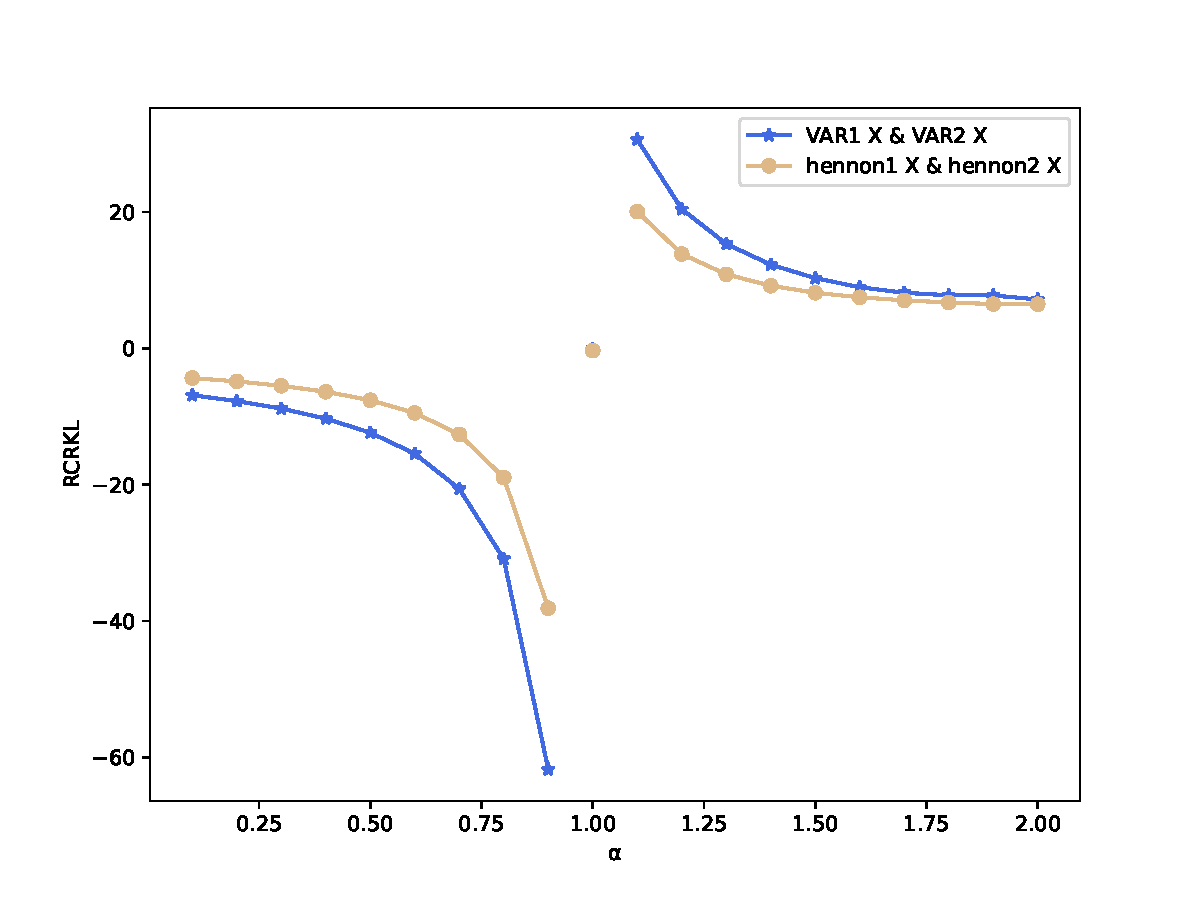
\includegraphics[scale=0.35]{./ch2/fig2_1.pdf}\label{a}
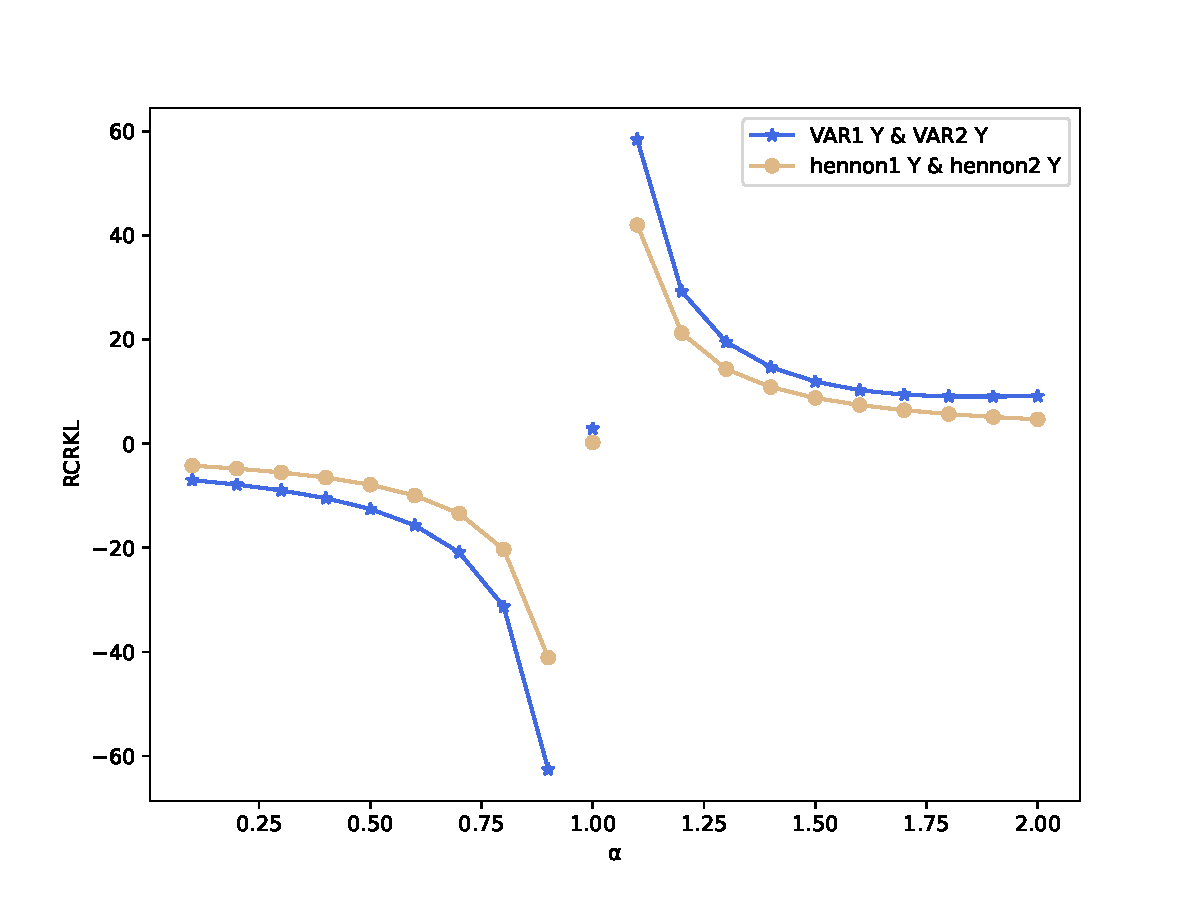
\includegraphics[scale=0.35]{./ch2/fig2_2.pdf}\label{b}
\caption{参数 $\alpha$ 对 $\rm{RCRKL}$ 的影响,图(a)为序列X之间的 $\rm{RCRKL}$, 图(b)为序列Y之间的 $\rm{RCRKL}$} \label{fig1}
\end{center}
\end{figure}\label{x_x_var}

为了验证 $\rm{RCRKL}$ 在测量两个时间序列差异方面的有效性。我们设计了一些合成数据对比实验。第一个实验是验证 $\rm{RCRKL}$ 在测量由不同系数的系统产生的序列之间的差异时的有效性。结果如图\ref{fig1}所示。图\ref{fig1}.a的曲线为$\rm{RCRKL(X_{VAR1}, X_{VAR2})}$和 $\rm{RCRKL(X_{\text{map}1}, X_{\text{map}2})}$。图\ref{fig1}.b的曲线为$\rm{RCRKL(Y_{VAR1}, Y_{VAR2})}$和$\rm{RCRKL(Y_{\text{map}1}, Y_{\text{map}2})}$。 正如我们在命题1中所证明的,当$\alpha\ge1$时,无论时序列X还是Y,各系统之间的$\rm{RCRKL}$都是正值,相反,当$0\le \alpha \le 1$时,各系统之间的$\rm{RCRKL}$则都是负值。此外,根据KL散度的理论,当 R\'enyi KL 散度为负时,意味着被比较的两个概率分布有重叠的支持,在结构上表现出相似性;当 R\'enyi KL 散度为正时,表明被比较的两个概率分布是不同的 \cite{22}。而根据R\'enyi熵理论\cite{17}. 当 $\alpha> 1$ 时,R\'enyi 熵更关注序列中的低频事件,而 $\alpha \in[0,1]$ 时,R\'enyi 熵更关注高频事件。因此,我们可以得出结论,对于VAR模型的趋势项(低频事件)来说,VAR1和VAR2是相似的。H'{e}non映射也同样存在这个现象。然而,在两个不同系数的 VAR 模型序列(或两个 \text{H'{e}non} 映射)之间,波动项(高频事件)的差异更大。相反,当 $\alpha=1$ 时,$\rm{RCRKL}$ 退化为传统的累积残差散度。从图中可以看出,不管是时间序列 $X$ 还是序列 $Y$,两个系统的 $\rm{CRKL}$ 差异都不大。而且正负性也不确定。同时,我们注意到 $\rm{RCRKL}$ 是随着 $\alpha$ 的增加而单调递减的,特别是当其取值在$(0.7,1)$ 和$(1,1.3)$ 时,$\rm{RCRKL}$ 的变化是显著的。因此,当使用 $\rm{RCRKL}$ 的任务对事件的相似性或差异性更为敏感时,$\alpha$ 的取值范围应为 $(0.7,1)$ 或 $(1,1.3)$。

\begin{figure}[htbp]
\begin{center}
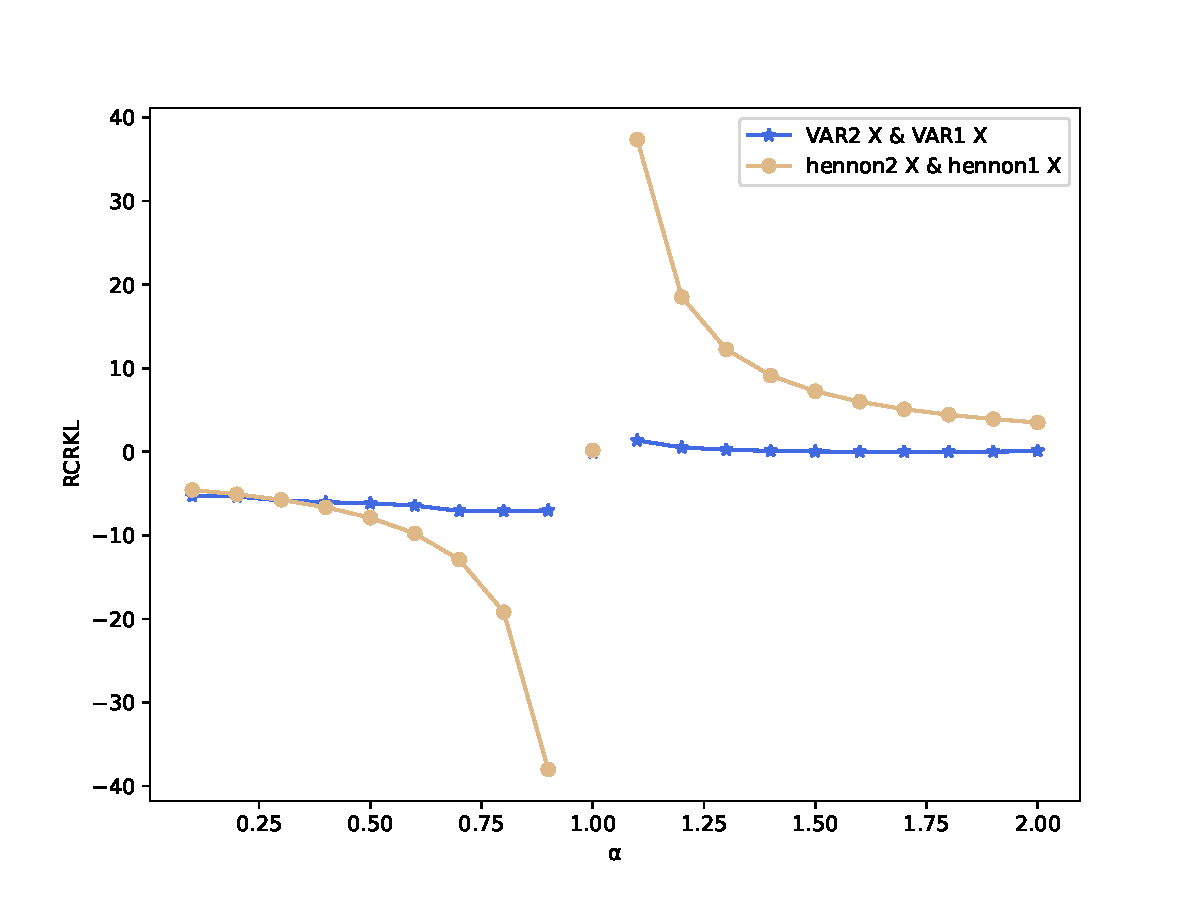
\includegraphics[scale=0.35]{./ch2/fig2_3.pdf}\label{a}
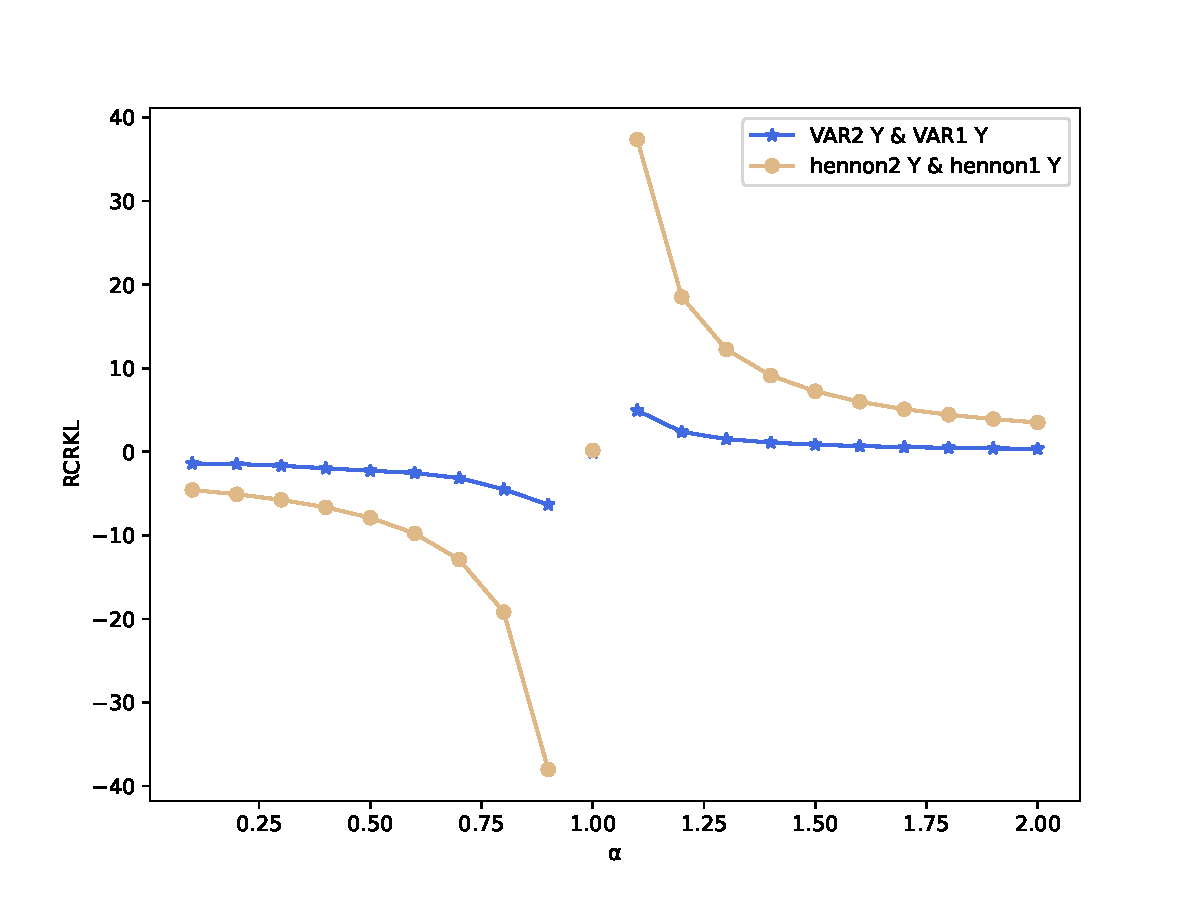
\includegraphics[scale=0.35]{./ch2/fig2_4.pdf}\label{b}
\caption{参数 $\alpha$ 对 $\rm{RCRKL}$ 的影响,图(a)为从VAR2到VAR1的 $\rm{RCRKL}$, 图(b)为从H\'{e}nnon map2 到 H\'{e}nnon map1的 $\rm{RCRKL}$} \label{fig2}
\end{center}
\end{figure}\label{x_y_var1}

由于 $\rm{CRKL}$ 是不对称的,这意味着 $\rm{RCRKL}(x,y) \neq \rm{RCRKL}(y,x)$。为了进一步说明 $\rm{CRKL}$ 的有效性,我们还比较了从 $\rm{VAR2}$ 到 $\rm{VAR1}$ 以及从 $\rm{text{H'{e}non}2}$ 到 $\rm{text{H'{e}non}1}$ 的 $\rm{RCRKL}$ 。结果如 图\ref{fig2} 所示,其中序列 $X$ 的 $\rm{RCRKL}$ 如图\ref{fig2}.a 所示,系列 $Y$ 的 $\rm{RCRKL}$ 如 图\ref{fig2}.b 所示。 与图 1 中的 $\rm{RCRKL}$ 结果相似,无论时序列X还是Y,从 $\rm{VAR2}$ 到 $\rm{VAR1}$ 以及从 $\rm{text{H'{e}non}2}$ 到 $\rm{text{H'{e}non}1}$ 的 $\rm{RCRKL}$ 都在 $\alpha\ge 1$ 时为负值,并且随着 $\alpha$ 的增大单调减小。同时,我们注意到在这种情况下,当$0<\alpha <1$时,$\rm{RCRKL}$ 的正负性是不确定的。从图 \ref{fig2}.b中$\rm{VAR2}$到$\rm{VAR1}$的$\rm{RCRKL}$可以看出,当$\alpha = 0.1$时,$\rm{RCRKL}$的值为正,当$\alpha \ge 0.1$时,$\rm{RCRKL}$的值变为负,这时,$\rm{RCRKL}$是与序列的分布有关的。

\subsection{关于 $\rm{RCRTE}$ 的仿真实验结果}


\begin{figure}[htbp]
\begin{center}
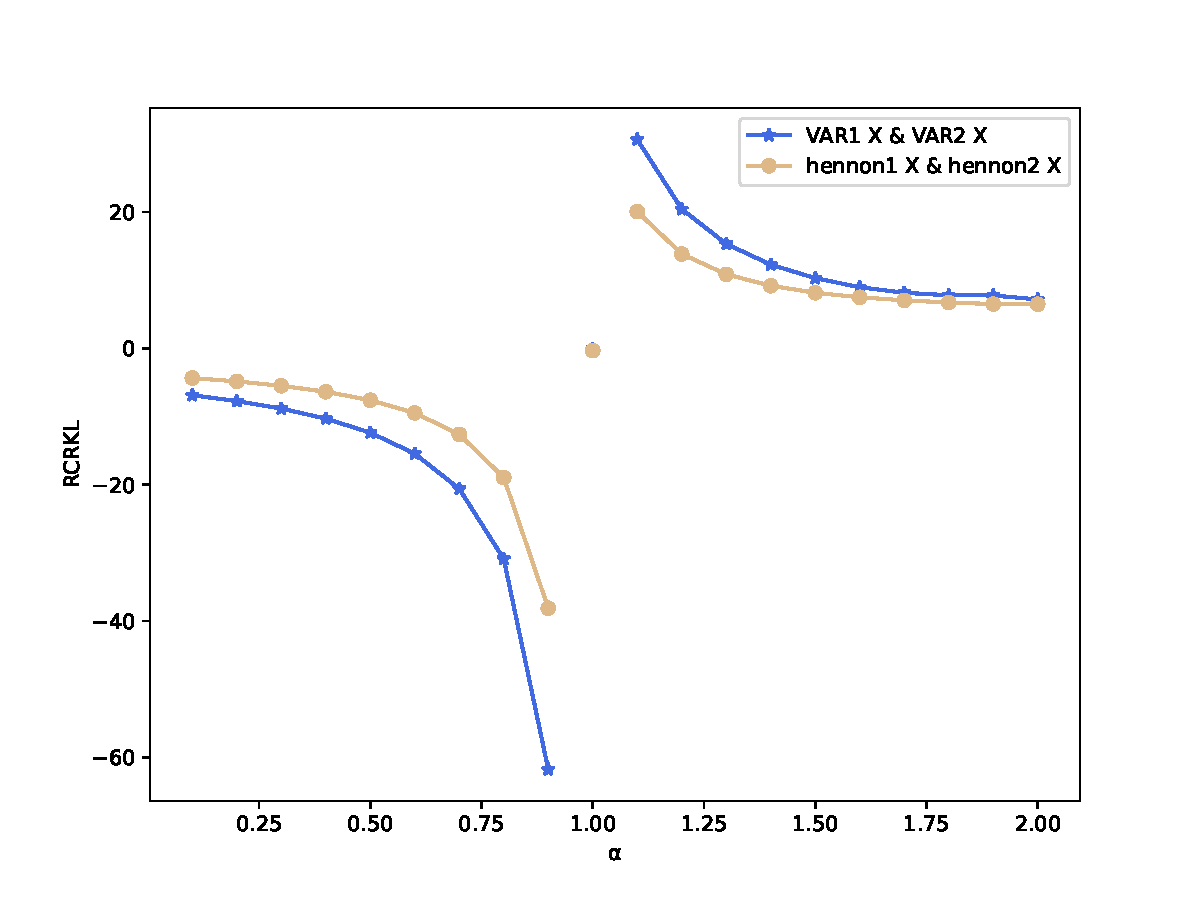
\includegraphics[scale=0.35]{./ch2/fig2_1.pdf}\label{a}
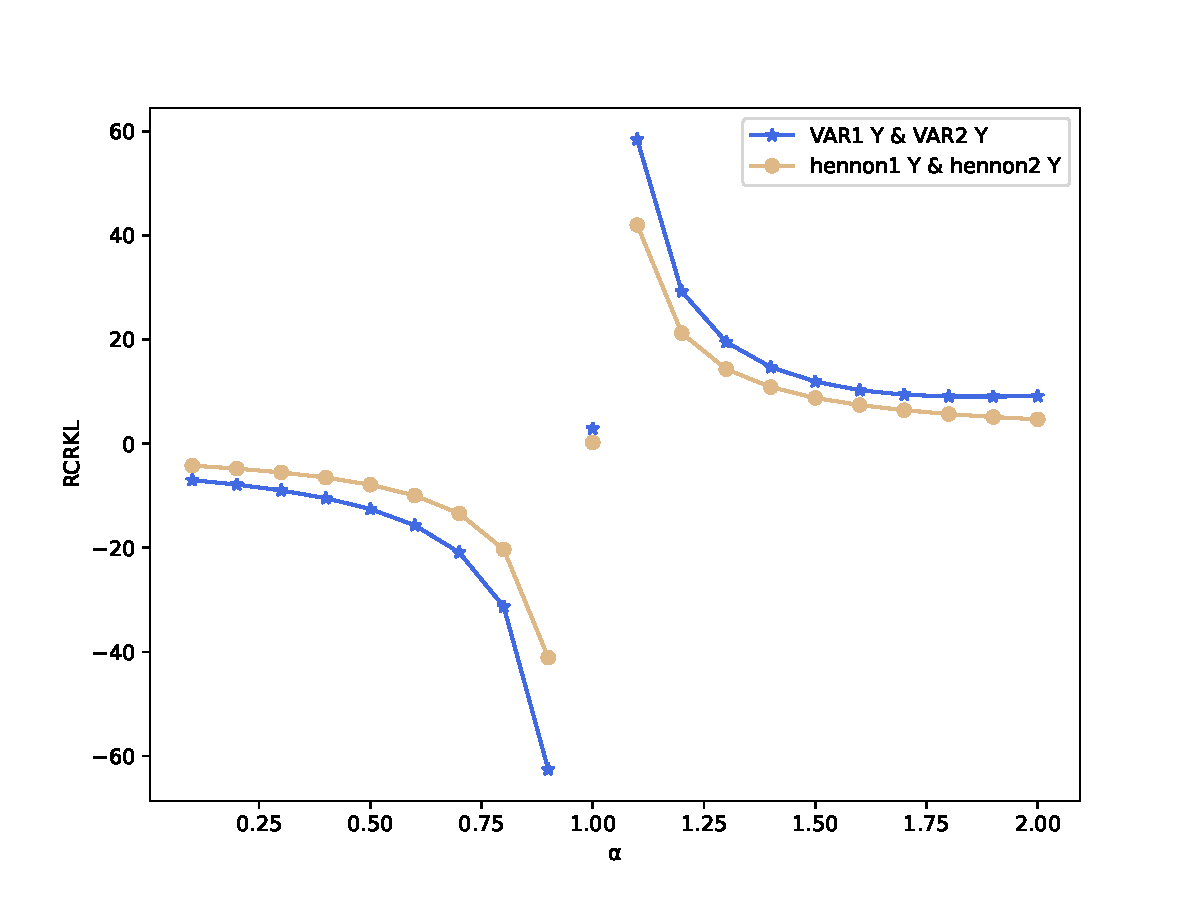
\includegraphics[scale=0.35]{./ch2/fig2_2.pdf}\label{b}
\caption{参数 $\alpha$ 对  VAR 模型和H\'{e}non映射的 $\rm{RCRTE}$ 值的影响。} \label{fig3}
\end{center}
\end{figure}\label{x_x_var}


$\rm{RCRTE}$ 是在R\'{e}nyi熵和累积残差熵的基础上对传递熵的扩展。它测量系统中变量序列之间的因果关系。为了验证本章提出的 RCRTE 的有效性,本节在合成数据上也进行了一些实验,不同于上一节有关$\rm{RCRKL}$上的实验,本节的实验均作用在系统内部,即序列X和Y之间。 在第一个实验中,我们验证$\alpha$对$\rm{RCRTE}$的影响,结果如图\ref{fig3}所示。在 $\rm{VAR1}$ 模型中,从系列 $X$ 到 $Y$ 的 $\rm{RCRTE}$ 如图\ref{fig3}.a 所示;在 $\rm{VAR2}$ 模型中,从系列 $X$ 到 $Y$ 的 $\rm{RCRTE}$ 如图.~\ref{fig3}.b 所示。结果表明,当 $\alpha \in (\infty, 1)$ 和 $(1,\infty)$ 时,$\rm{RCRTE}$ 分别随 $\alpha$ 的增加而单调递减。同时,正如命题 6 所证明的那样,$\rm{RCRKL}\neq 0$,因为 $X$ 和 $Y$ 的分布并非处处相等。这一特性可以帮助我们在因果检测中剔除没有时间依赖性或信息流的变量。


\begin{figure}[htbp]
\begin{center}
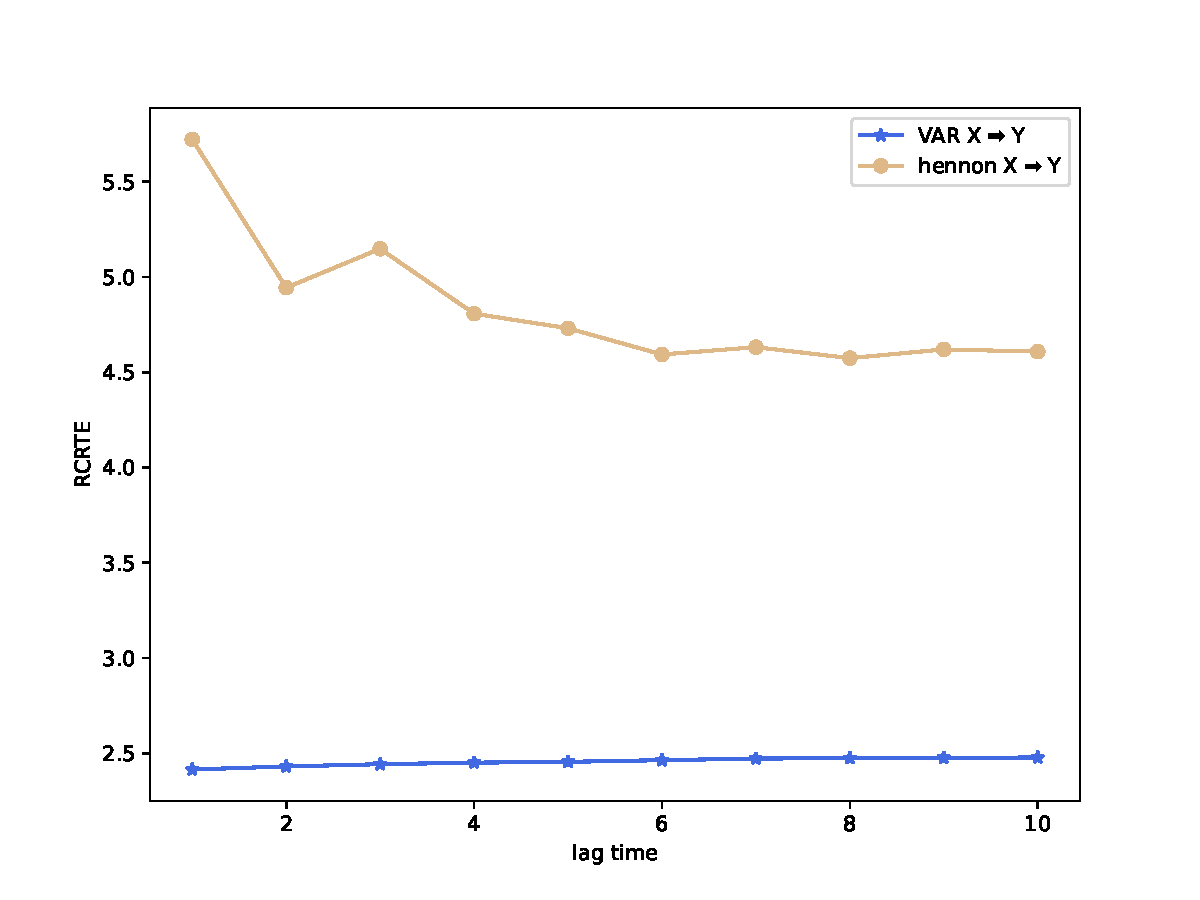
\includegraphics[scale=0.35]{./ch2/fig2_7.pdf}\label{a}
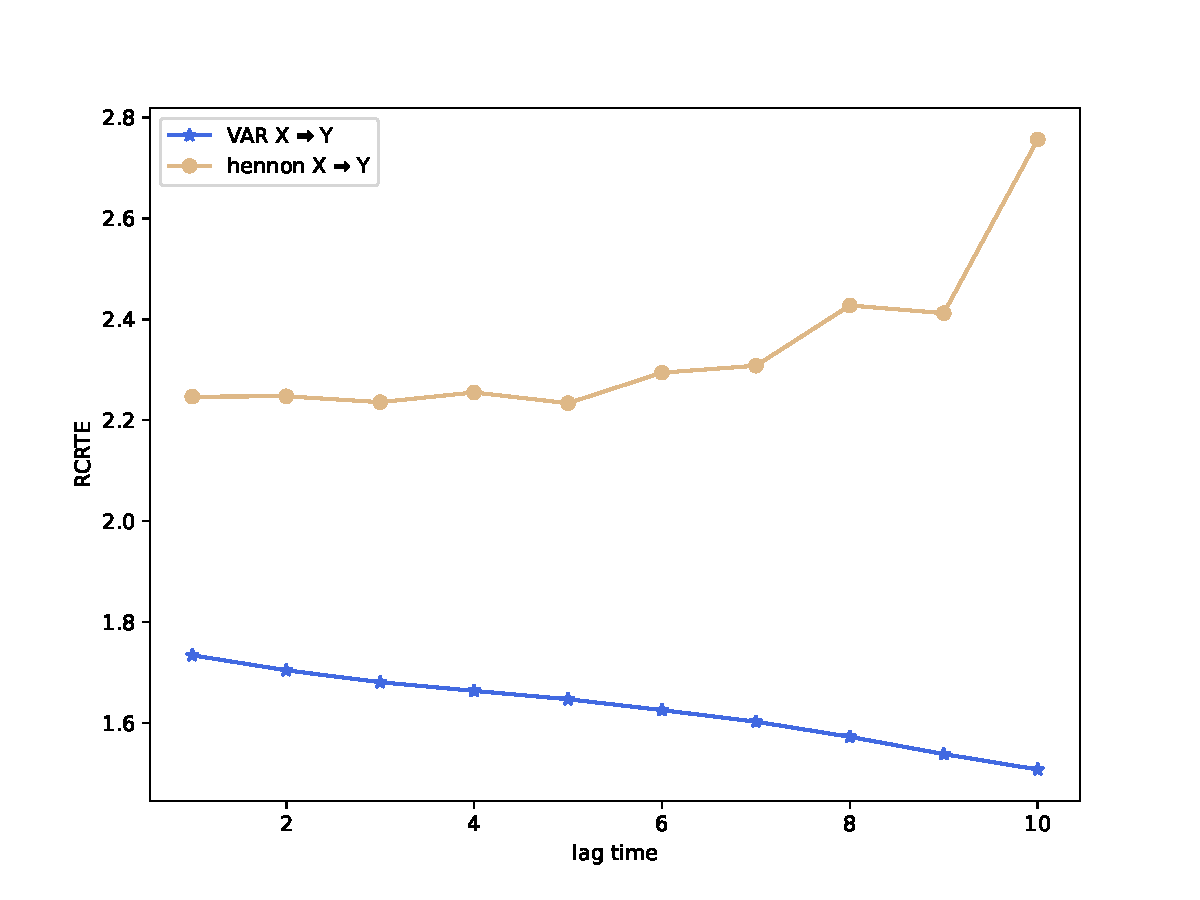
\includegraphics[scale=0.35]{./ch2/fig2_8.pdf}\label{b}
\caption{滞后时间 $l$ 和 $k$ 对 VAR 模型和H\'{e}non映射的 $\rm{RCRTE}$ 值的影响。} \label{fig4}
\end{center}
\end{figure}\label{x_y_var2}


马尔可夫阶数 $l$ 和 $k$ 是另一个会影响 $\rm{RCRTE}$ 值的参数。它决定了用于计算 $t$ 时刻 $\rm{RCRTE}$ 的 $X$ 序列和 $Y$ 序列历史信息的长度。图 \ref{fig4}直观地展示了马尔可夫阶数对$\rm{RCRTE}$值的影响。为方便起见,将 $l$ 和 $k$ 设置为相同值,范围为:$l=k \in [1, 10]$。总的来说,无论 $\alpha$ 是否大于 1,两个系统的 $\rm{RCRTE}(X/rightarrow Y)$ 都是正值。这表明,无论是长尾事件还是普通事件,$X$都是$Y$的因果源。此外,马尔可夫阶数对 VAR 模型和 h\'{e}non映射的影响也不尽相同。具体来说,VAR 模型的 $\rm{RCRTE}$ 值在两个方向上都是稳定的,而 H\'{e}nnon 映射 的 $\rm{RCRTE}$ 值在而当 $l\in [3,10]$ 时两个方向上都是相对稳定的,变化幅度较小,而当 $l \in[1,2]$ 时,$\rm{RCRTE}(X\rightarrow Y)$ 值有快速下降的趋势,当 $l>9$ 时,$\rm{RCRTE}(Y\rightarrow X)$ 值快速上升。不同的结果意味着,在处理不同系统时,发生统计意义上的因果相关性的历史序列长度是不同的,而且需要谨慎选择马尔可夫阶。

\section{实例应用}
本章的实例数据来自RIOHTrack数据集,有关该数据集的详细介绍在第一章中已经给出,本章不在赘述。这里介绍一下本章所使用数据,车辙及其影响因素被选用来验证 $\rm{RCRKL}$ 和 $\rm{RCRTE}$ 的有效性,影响因素包括温度、荷载量和中心点弯沉。路面分为19组结构,每组结构144个数据点。

RIOHTrack 车辙实验分为两部分:1.基于 $\rm{RCRKL}$ 的车辙时间序列聚类;2.基于 $\rm{RCRTE}$ 的车辙因果分析。实验的流程设计如下: 在第一部分中,基于 $\rm{RCRKL}$ 对 19 个路面车辙的时间序列进行分层聚类,将其聚成相似的簇。对于每个聚类,在第二部分中通过 $\rm{RCRTE}$ 检测车辙与其影响因素之间的因果关系。

\subsection{基于 $\rm{RCRKL}$ 的车辙时间序列聚类结果及讨论}
本节提出了一种基于 $\rm{RCRKL}$ 的新型 k-means 聚类方法,其中用 $\rm{RCRKL}$ 代替了欧式距离度量。在第二节中,我们证明了当 $\alpha > 1$ 时,$\rm{RCRKL}$ 是非负的,并且三角形不等式在 $\rm{RCRKL}$ 上成立,然而,由于其不对称性,$\rm{RCRKL}$ 不能直接被用作距离度量,即 $\rm{RCRKL}(X,Y) \neq \rm{RCRKL}(Y,X)$。为了解决这个问题,本文设计了一种基于 $\rm{RCRKL}$ 的对称距离度量:
\begin{align*}
D_{RCRKL}(X,Y) = \frac{RCRKL(X,Y)+RCRKL(Y,X)}{2}.
\end{align*}
显然,$\rm{D_{RCRRKL}(X,Y)}$ 是对称的,即 $\rm{D_{RCRKL}(X,Y)} = \rm{D_{RCRRKL}(Y,X)}$。因此,基于 $\rm{RCRKL}$ 的距离度量已被完整定义,在此基础上,我们可以使用已有的聚类算法对时间序列进行聚类。作为一种典型的无监督聚类算法,AP 聚类在本节中被使用,其设计算法为 \ref{alog 1}:
\begin{algorithm}[htbp]
\caption{基于$\rm{RCRKL}$的AP聚类} \label{alog 1}
\label{alg:SA1}

\begin{algorithmic}[1]
    % Step 1: Initialization
\STATE \textbf{输入:}
\STATE - 多元时间序列 $X_n$
\STATE - 最大迭代次数 $max\_iterations$

\STATE \textbf{初始化:}
\STATE -  将可用矩阵 $A$ 初始化为零矩阵
\STATE - 将责任矩阵 $R$ 初始化为零矩阵

\STATE \textbf{信息传递:}
\FOR{each iteration \textbf{from} 1 \textbf{to} $max\_iterations$}
    \FOR{each time series $i$ \textbf{from} $X_1$ \textbf{to} $X_n$}
        \FOR{each time series $j$ \textbf{from} $X_1$ \textbf{to} $X_n$ except $i$}
            \STATE 通过下列公式计算责任矩阵 R(i, j):
            \STATE $R(i, j)=(\rm{RCRKL}(x_i, x_j)+\rm{RCRKL}(x_j, x_i)) / 2-\max(A(i, :)+(\rm{RCRKL}(x_i, x_j)+\rm{RCRKL}(x_j, x_i)) / 2 \text{ except for } R(i, j))$
        \ENDFOR
    \ENDFOR

    \FOR{each time series $i$ \textbf{from} 1 \textbf{to} $X_n$}
        \FOR{each time series $j$ \textbf{from} 1 \textbf{to} $X_n$}
            \STATE 通过下列公式计算可用矩阵 $A(i, j)$ :
            \STATE $A(i, j) = \min(0, R(j, j) + \sum(\max(0, R(k, j)) \text{ except for } i \text{ and } j))$
        \ENDFOR
    \ENDFOR
\ENDFOR

\STATE \textbf{范例点和簇的确定:}
\STATE - 通过查找具有正净责任的数据点来确定范例点: (sum of $R(i, i)$ and $A(i, i)$)
\STATE - 将每个数据点分配到与其最近的示例相关联的簇中

\STATE \textbf{输出:}
\STATE - 范例点及其相应的簇

\end{algorithmic}
\end{algorithm}

算法\ref{alog 1}的聚类可视化结果如图\ref{fig2_9}所示。聚类结果如下: STR1-STR5 的车辙在第 1 簇,STR6-STR9 的车辙在第 2 簇,STR10-STR11 的车辙在第 3 簇,STR12-STR14 的车辙在第 4 簇,其余车辙在第 5 簇。由于 AP 算法是一种无监督算法,因此不存在聚类结果的绝对正确结果。为了便于比较,我们参考了一些工程经验分类结果。根据 RIOHTrack 之前的研究,路面结构设计可以根据沥青层的组合和厚度分为 5 组,如表\ref{table1}所示。与基于结构的分类相比,基于 $\rm{RCRKL}$ 的 AP 算法的结果在聚类数量上是相同的,都是 5 个。但是,基于所提聚类算法的每个聚类中的元素与基于经验的路面结构类别并不相同。主要区别在于,半刚性基层结构中的路面被分为 STR1-STR3 和 STR6-STR9 两组,而倒置结构中的 STR10 和 STR12 则被分为不同的簇。针对这一现象,一些基于复杂网络分析的研究表明,作为粘弹性半刚性体,路面的变形与沥青的厚度有关。这一解释反映在聚类结果中,即具有相似沥青层厚度的路面更有可能聚类在同一个聚类中\cite{29}。


\begin{figure*}[htbp]
\begin{center}
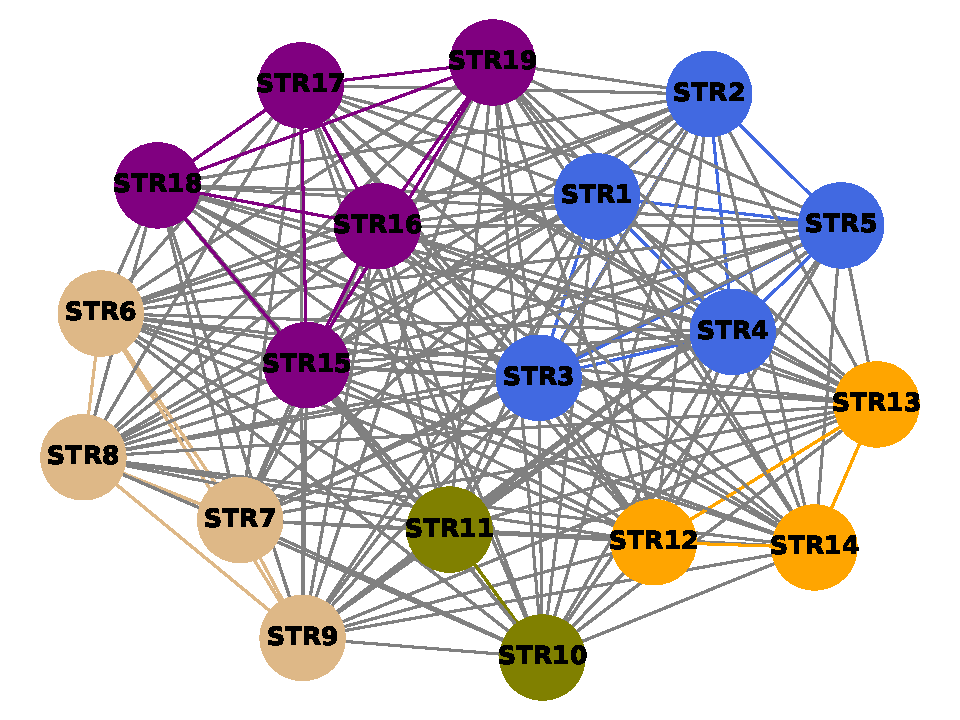
\includegraphics[scale=0.5]{./ch2/fig2_9.pdf}
\caption{基于 $\rm{RCRKL}$ 的 AP 聚类算法得出的 RIOHTrack 车辙时间序列聚类结果} \label{fig3}
\end{center}
\end{figure*}

\begin{table}[!ht]
\fontsize{8}{14}\selectfont
\centering
\caption{基于经验设计的 RIOHTrack 路面结构分类。}
\begin{tabular}{lll}
 \hline
 簇编号 &  路面类别 & 路面编号\\
  \hline
  1 &  semi-rigid base structure & STR1-STR3, STR6-STR9\\
  \hline
  2 &  rigid base structure & STR4, STR5\\
  \hline
  3 &  inverted structure & STR10, STR12\\
  \hline
  4 &  flexible base structure & STR11, STR13-STR17\\
  \hline
  5 &  full thickness structure & STR18, STR19\\
  \hline
\end{tabular}
\label{table1}
\end{table}

此外,为了验证基于 $\rm{RCRKL}$ 的聚类算法的性能,本节还对基于不同距离度量的聚类算法进行了比较。我们将重点限制在应用于时间序列的方法上,即皮尔逊相关性(Pearson Correlation,PC)\cite{30}、动态时间扭曲(Dynamic Time Warping,DTW)\cite{31}和马哈拉诺比斯距离(Mahalanobis Distance,MD)\cite{32}。性能评估指标是一些内在的衡量标准: 剪影系数(Silhouette Coefficient,SC)、戴维斯-博尔丁指数(Davis Boulding Index,DBI)和邓恩指数(Dunn Index,DI)。SC 计算的是所有时间序列点的平均剪影系数,其中点的剪影系数被定义为与自身聚类中点的平均距离和与最近相邻聚类中点的平均距离之差。SC 越高,表示聚类越清晰。DB 指数评估聚类之间的紧凑性和分离度。它被定义为每个聚类与其最相似聚类之间的平均相似度。DBI 指数越低,表示聚类越清晰、分离度越高。DI 衡量聚类的紧凑程度(聚类内距离)和聚类间的分离程度(聚类间距离)。DI 值越高,表示聚类质量越好。本次验证中使用的所有距离指标均为 $\rm{RCRKL}$。

总体而言,基于 $\rm{RCRKL}$ 的聚类算法的性能优于其他方法。特别是在 SC 测量中,本文提出的聚类算法表现较好,SC($\rm{RCRKL}$) = 0.43,表明聚类结果合理,聚类之间的分离度适中。在 DB 的测量中,只有 DB($\rm{RCRKL}$)=0.37 和 DB($\rm{DTW}$)=0.27 小于 0.5。结果表明,聚类结果相对较好,聚类分离度较高。最后,基于 $\rm{RCRKL}$ 的聚类算法的 DI 值为 0.5,这表明聚类结果具有良好的分离性。

\begin{table}[!ht]
\fontsize{8}{14}\selectfont
\centering
\caption{基于不同距离度量的 AP 算法的平均内在测量值比较。}
\begin{tabular}{llll}
 \hline
 距离度量 &  SC & DBI & DI\\
  \hline
  PC &  -0.03 & 1.12 &0.18\\
  \hline
  DTW &  0.27 & 0.49 &0.35\\
  \hline
  MD &  0.15 & 0.63 &0.22\\
  \hline
  RCRKL &  0.43 & 0.37 &0.50\\
  \hline
\end{tabular}
\label{table2}
\end{table}

\subsection{基于 $\rm{RCRTE}$ 的车辙时间序列因果检测结果及讨论}
最后,我们分析了 5 个群组内车辙影响因素的 $\rm{RCRTE}$ 值。对于参数 $\alpha$ ,我们选择了两个值,分别为 $\alpha=0.5$ 和 $\alpha=1.5$ ,分别对应于时间序列中的低概率事件和高概率事件。滞后时间 $l=k=5$ 的结果如图\ref{fig7}和图\ref{fig8}所示。很明显,从挠度盆深度到车辙的$\rm{RCRTE}$在两个$\alpha$值上均为正,这说明路面刚度是车辙的重要成因。同时,大多数聚类上从路面温度到车辙的 $\rm{RCRTE}$在 $\alpha\le1$时为负值,而在聚类 1 上,当 $\alpha \ge 1$时为正值。这表明对于长尾事件,如车辙的快速加深,温度变化是其因果来源,而对于普通事件,如车辙的平稳发展,温度不应被视为因果来源。具体来说,对于属于第 1 组和第 2 组的半刚性基层结构路面和刚性基层结构路面,在长尾事件中,温度是车辙产生的原因,而在普通事件中,交通荷载是车辙产生的原因。对于属于第 3 组和第 4 组的厚沥青混凝土基层结构路面,交通荷载也是长尾事件车辙产生的原因。而对于属于第 5 组的全深度沥青混凝土结构路面,温度是长尾事件和普通事件车辙产生的原因。同时,我们还注意到,在某些群组中,从温度和交通荷载到挠度盆深度的 $\rm{RCRTE}$ 也是正值,这意味着这两个因素在某些情况下会影响路面刚度。
\begin{figure*}[htbp]
\begin{center}
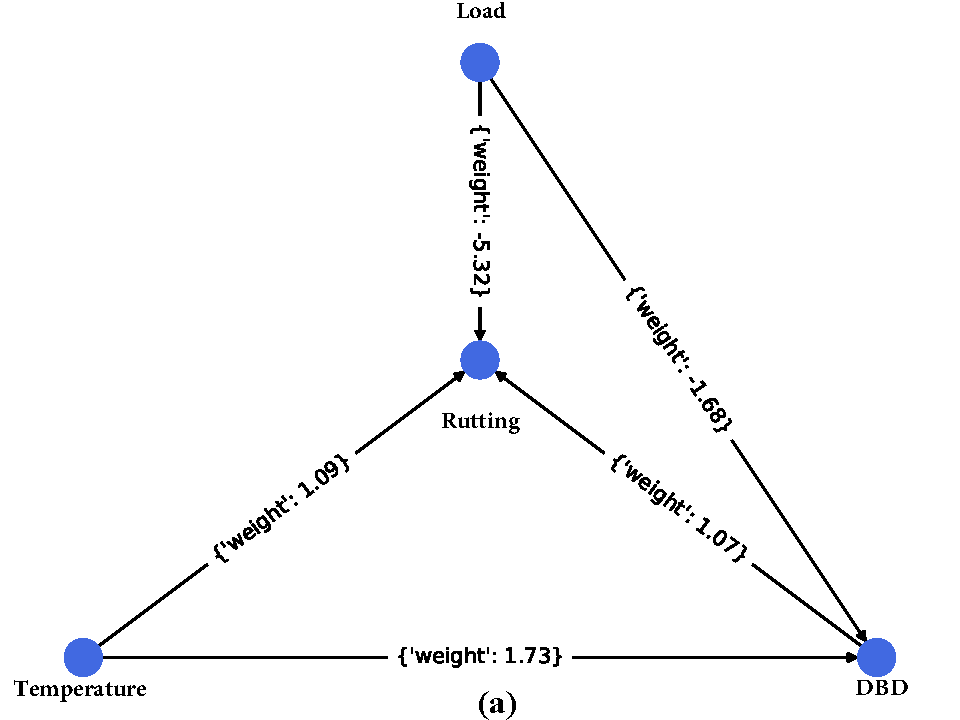
\includegraphics[scale=0.3]{./ch2/fig2_11.pdf}
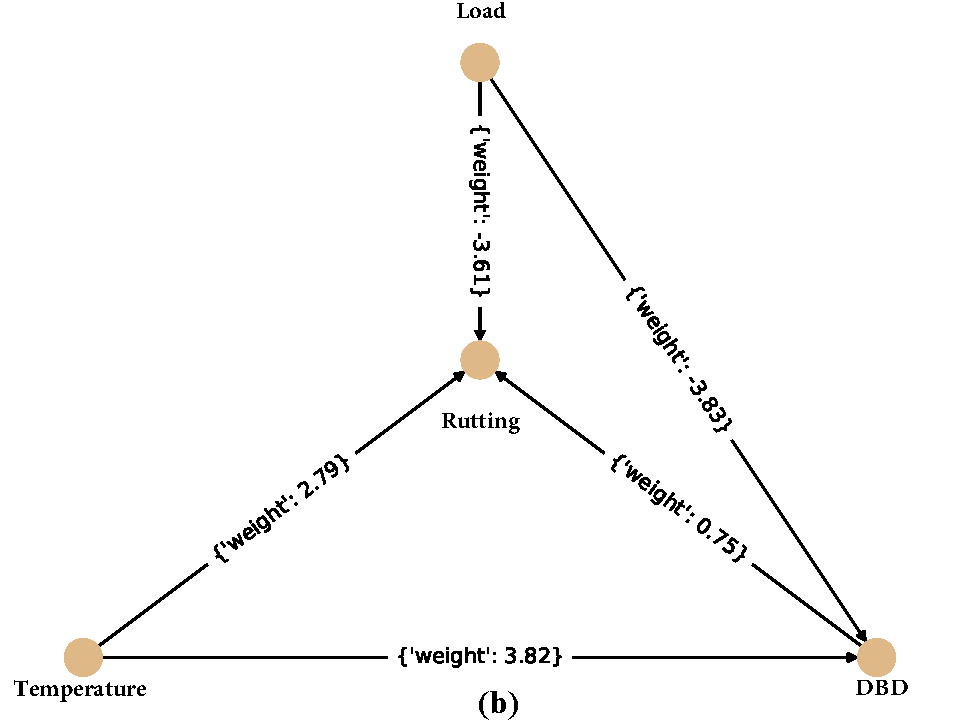
\includegraphics[scale=0.3]{./ch2/fig2_12.pdf}
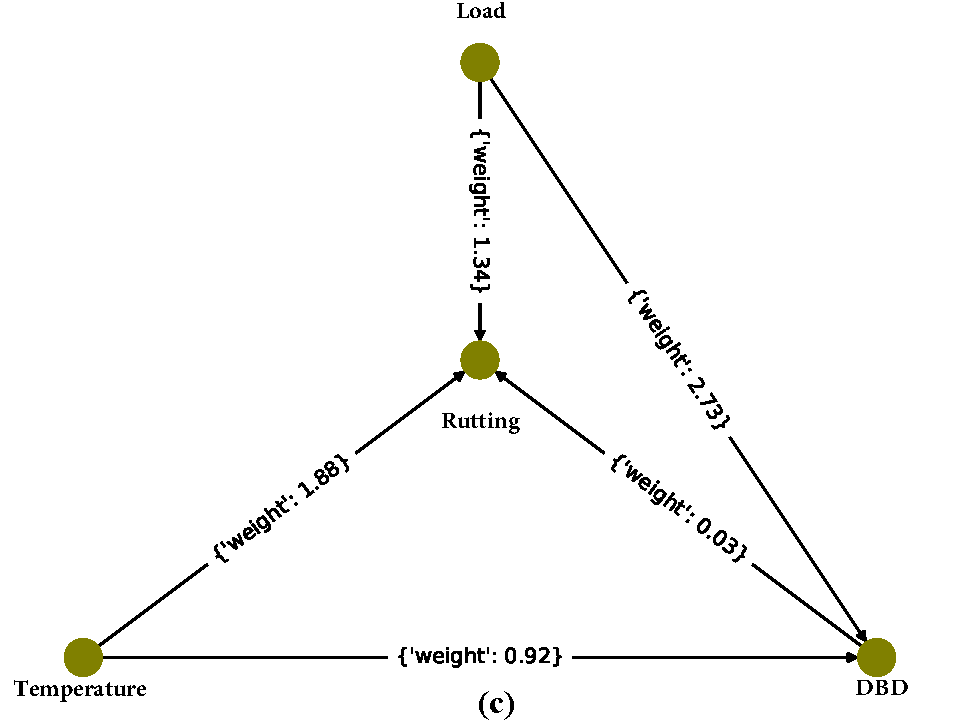
\includegraphics[scale=0.3]{./ch2/fig2_13.pdf}\\
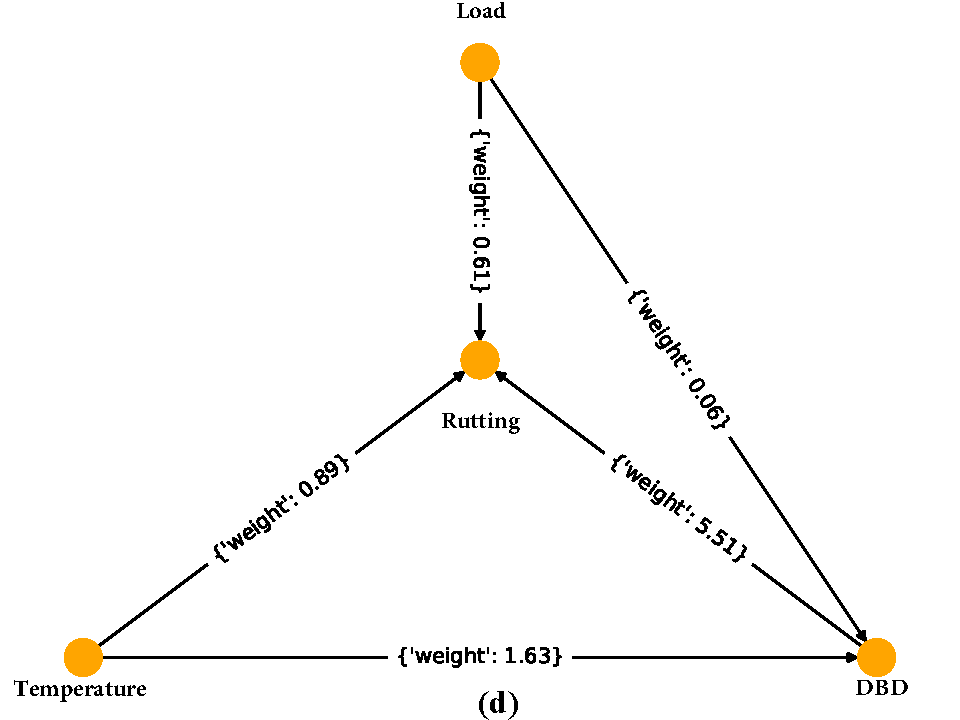
\includegraphics[scale=0.3]{./ch2/fig2_14.pdf}
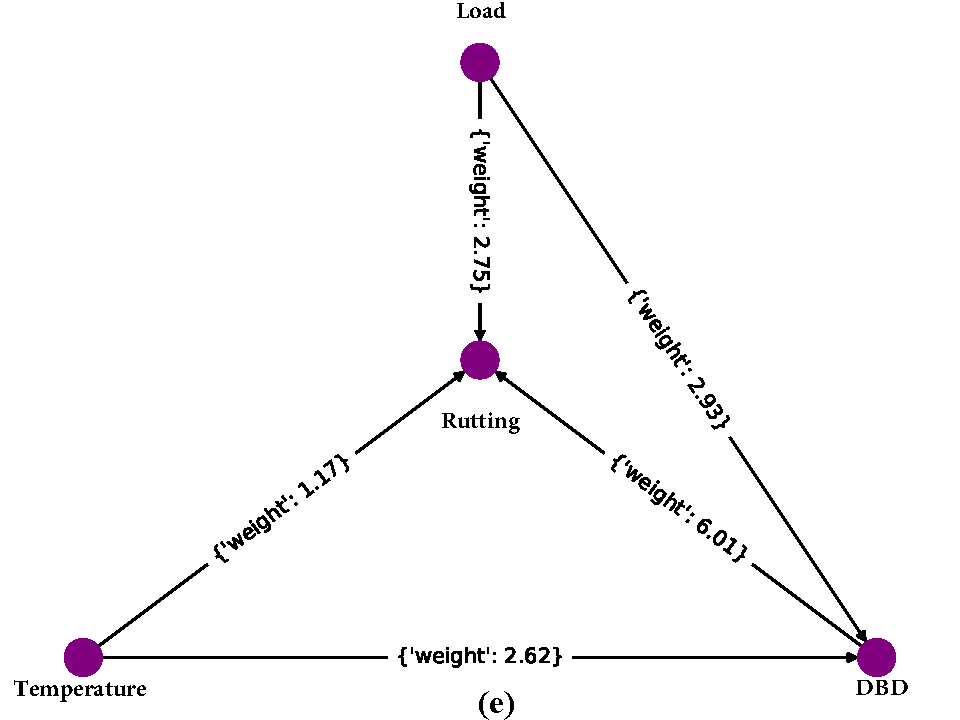
\includegraphics[scale=0.3]{./ch2/fig2_15.pdf}
\caption{5 个聚类上从影响因素到车辙的 $\rm{RCRTE}$ 值图表可视化,其中参数为 $\alpha=0.5$,$l=k=2$。} \label{fig7}
\end{center}
\end{figure*}

\begin{figure*}[tbp]
\begin{center}
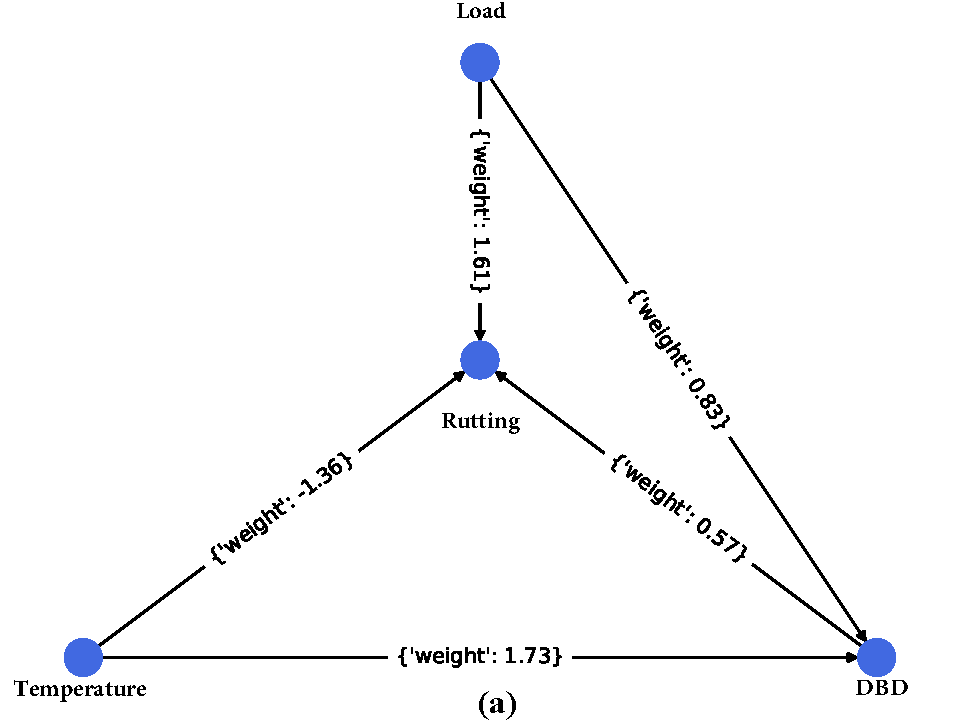
\includegraphics[scale=0.3]{./ch2/fig2_16.pdf}
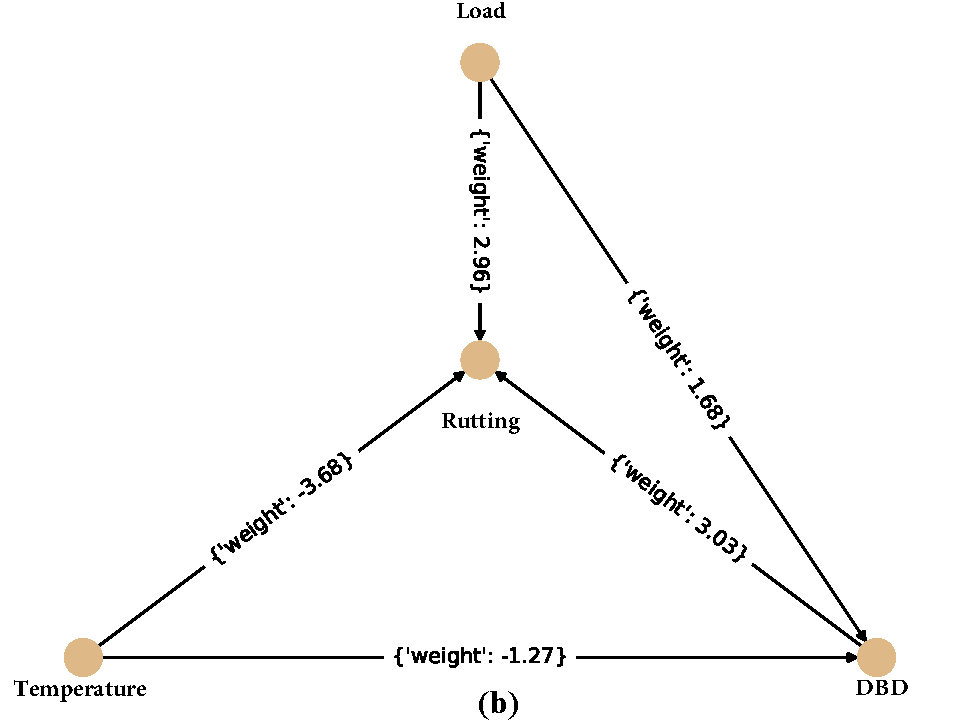
\includegraphics[scale=0.3]{./ch2/fig2_17.pdf}
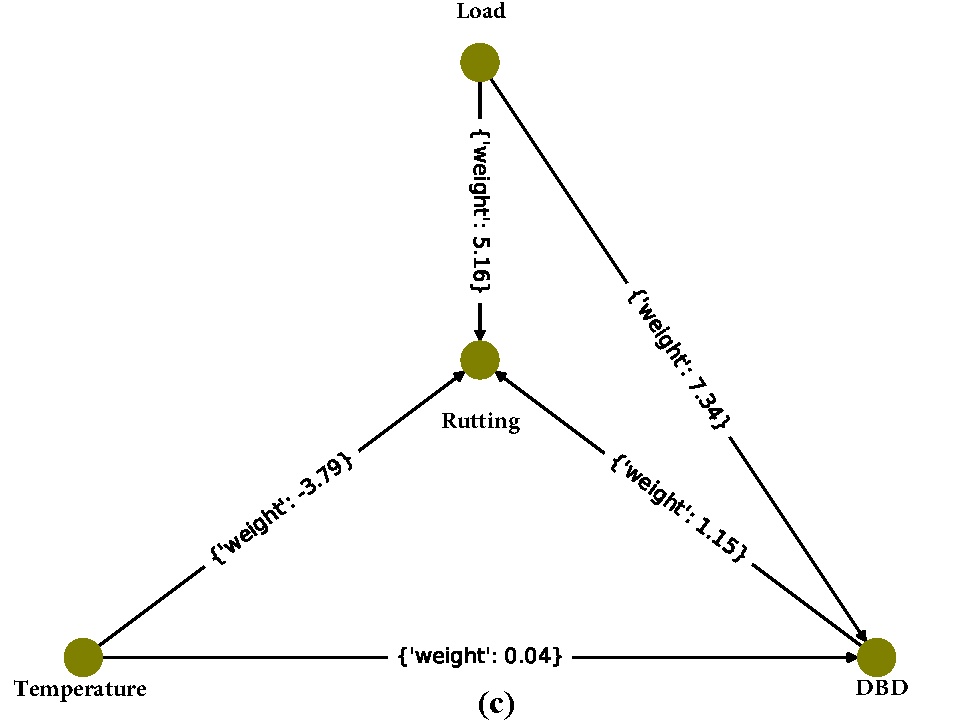
\includegraphics[scale=0.3]{./ch2/fig2_18.pdf}\\
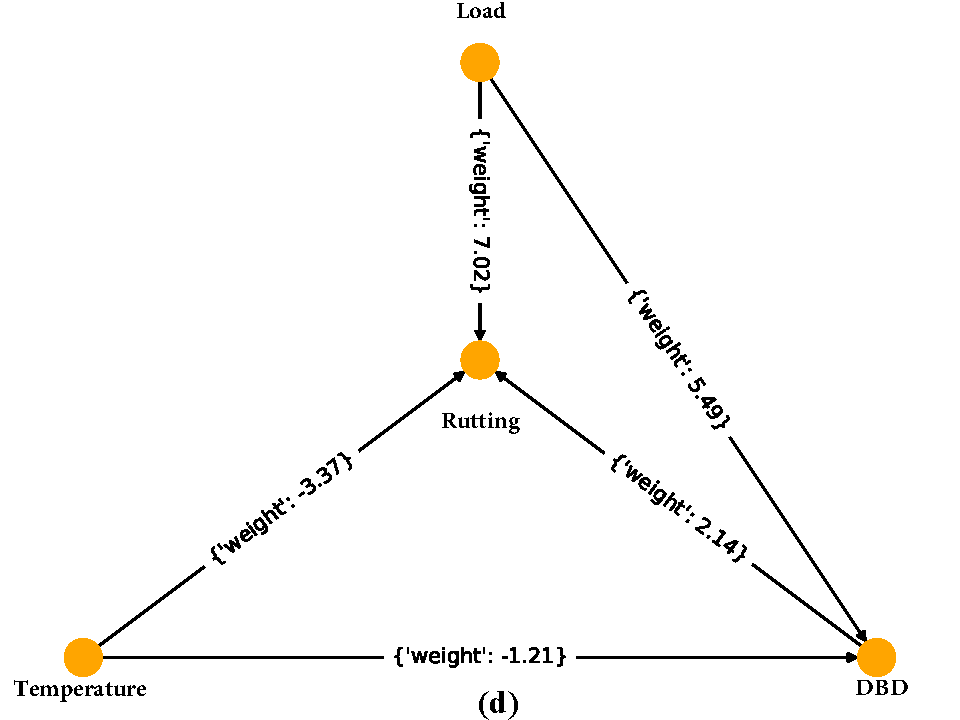
\includegraphics[scale=0.3]{./ch2/fig2_19.pdf}
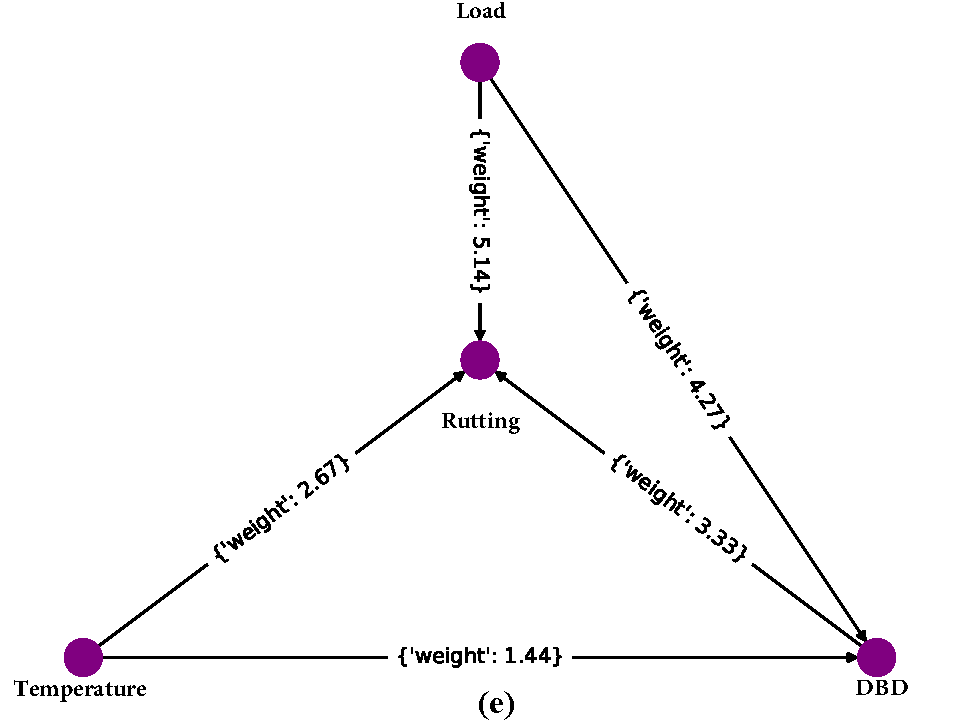
\includegraphics[scale=0.3]{./ch2/fig2_20.pdf}
\caption{5 个聚类上从影响因素到车辙的 $\rm{RCRTE}$ 值图表可视化,其中参数为 $\alpha=1.5$,滞后时间为 $l=k=2$。} \label{fig8}
\end{center}
\end{figure*}

与经典 TE 相比,分数 $\rm{RCRTE}$ 可以在分数阶 $\alpha$ 的范围内更全面地检测影响因素与车辙之间的因果关系。

\section{小结} 
本文引入了两种新的分数阶时间序列度量--R\'{e}nyi累积残差KL散度(R\'{e}nyi cumulative residual Kullback-Leibler,$\rm{RCRKL}$)和R\'{e}nyi累积残差转移熵(R\'{e}nyi cumulative residual transfer entropy,$\rm{RCRTE}$)。研究并证明了 $\rm{RCRKL}$ 和 $\rm{RCRTE}$ 的一些数学性质。我们证明了 $\rm{RCRKL}$ 作为距离度量的一些性质。并研究了 $\rm{RCRTE}$ 的零点和边界。然后,我们提供了一些仿真数据的例子来研究参数变化对度量值的影响。最后,将两个分数阶时间序列度量应用于路面车辙时间序列,设计了基于 $\rm{RCRKL}$ 的AP聚类,并通过 $\rm{RCETE}$ 检测了影响因素与车辙之间的因果关系。总的来说,本章所提出的 $\rm{RCRKL}$ 和 $\rm{RCRTE}$ 兼具了 $\rm{CRE}$ 和 $\rm{RE}$ 的优点,同时对时间序列的度量提供了更加全面的见解和分析。在未来的工作中,我们将进一步把这两个度量应用到其他领域的时间序列数据中以验证它们的泛化性,同时,基于诸如Tsallis熵这样的分数阶熵,将这两个度量进一步扩展到更多形式的分数阶度量以增加它们的全面性。
本章结果已发表在国际刊物  Neural Networks 上。具体详见作者发表论文的清单。
